% ------------------------------------------------------------------------
% -------------------      Plantilla_UIS.tex       -----------------------
% ------------------------------------------------------------------------
% ------------------------------------------------------------------------
% Versión de plantilla para realización de informes de trabajo de grado
% construida para uso de la Universidad Industrial de Santander.
%
% Reservados todos los derechos
%
% Bucaramanga, Colombia
% Febrero 03 de 2019
%
% ------------------------------------------------------------------------
% ------------------------------------------------------------------------

\documentclass[letter,oneside,12pt,spanish]{report}  % Encabezados
\usepackage[utf8]{inputenc}

\usepackage[spanish,es-nodecimaldot]{babel}
\usepackage{booktabs}
\usepackage{uislatexstyleAPA}
\usepackage{verbatim} 
% Libreria UIS APA
% ------------------------------------------------------------------------
% Ingrese en este punto las librerías específicas de usuario
% -----------------------------------------------------------------------

\usepackage{amsmath, amsfonts}
\usepackage{epsfig}
\usepackage{amsmath}
\usepackage{amssymb}
\usepackage{subfigure}
\usepackage{float}
\usepackage{ragged2e}
\usepackage{graphicx}
\usepackage[table,xcdraw]{xcolor}
\usepackage{multirow}
%\usepackage{url}


% Inicio de documento
% -------------------------------------------------------------------
\begin{document}
% Inicio de documento
% ------------------------------------------------------------------------
% Definición silábica de palabras
% ------------------------------------------------------------------------
%\hyphenation{pro-por-cio-nal di-se-ño}
% ------------------------------------------------------------------------
% Titulo resumido del trabajo que aparecerá en cornisa
%https://www.overleaf.com/project/5e82cd0e525d6d00011cf82f% ------------------------------------------------------------------------
\title{REGISTRO DE EVENTOS PROYECTO LAGO}
% ------------------------------------------------------------------------
% Elementos previos al contenido del trabajo
% ------------------------------------------------------------------------
% ------------------------------------------------------------------------
%                               Portadilla
% ------------------------------------------------------------------------

\begin{center}

IMPLEMENTACI\'ON DE UN SISTEMA PARA EL REGISTRO DE EVENTOS RELACIONADOS CON RAYOS C\'OSMICOS SECUNDARIOS\vfill%\vspace{0.8cm}

Dora Luz Ballesteros Delgado%\vspace{0.8cm}

Trabajo de Grado para optar al t\'itulo de Ingeniera Electr\'onica\vfill %\vspace{0.8cm}

Director\\
Carlos Andr\'es Angulo Julio\\
Magíster en Ing. Electr\'onica\bigskip

%\vspace{0.8cm}
Codirectores\\
Luis Alberto Núñez de Villavicencio Martínez \\
Ph.D  Física \bigskip

Jesús Peña Rodríguez\\
Ph.D (c) en F\'isica
\vfill
%\vspace{0.8cm}

Universidad Industrial de Santander\\
Facultad de Ingenier\'ias Fisicomec\'anicas\\
Escuela de Ingenier\'ias El\'ectrica, Electr\'onica y de Telecomunicaciones\\
Bucaramanga\\
2020
\end{center}

% ------------------------------------------------------------------------
%                             Nota de proyecto
% ------------------------------------------------------------------------
%\newpage

%\begin{figure}
%\centering
%
\includegraphics[width=0.85\textwidth]{Figs/nota}
%
\includegraphics[width=0.9\textwidth,draft]{Figs/nota}
%\end{figure}

% ------------------------------------------------------------------------
%                             Autorización
% ------------------------------------------------------------------------
%\newpage

%\begin{figure}
%\centering
%
\includegraphics[width=0.85\textwidth]{Figs/autoriza}
%
\includegraphics[width=0.9\textwidth, draft]{Figs/autoriza}
%\end{figure}
% ------------------------------------------------------------------------              % Portadilla, formato de nota y autorización
% ------------------------------------------------------------------------
% ------------------------------------------------------------------------
% ------------------------------------------------------------------------
% ------------------------------------------------------------------------
%                               Dedicatoria
% ------------------------------------------------------------------------
% ------------------------------------------------------------------------
% ------------------------------------------------------------------------
\chapter*{Dedicatoria}


% ------------------------------------------------------------------------                                    % Dedicatoria
% ------------------------------------------------------------------------
% ------------------------------------------------------------------------
% ------------------------------------------------------------------------
% ------------------------------------------------------------------------
%                             AGRADECIMIENTOS
% ------------------------------------------------------------------------
% ------------------------------------------------------------------------
% ------------------------------------------------------------------------
\chapter*{Agradecimientos}

\noindent Agradezco a mi familia por el apoyo ecónomico y moral que tuvieron para conmigo
durante el desarrollo de mi carrera. También agradezco a mis amigos y
compañeros por las vivencias de estos inolvidables años de universidad.\\

Un reconocimiento y agradecimiento importante lo realizo a mi director de
trabajo de grado, por dedicar su tiempo, experiencia y conocimiento en la guía
de mi proyecto.
% ------------------------------------------------------------------------
\newpage                            % Agradecimientos
% ------------------------------------------------------------------------
\tableofcontents                                      % Tabla de contenido
% ------------------------------------------------------------------------
\listoffigures                         % Lista de figuras, tablas y anexos
\listoftables
%\listofanexo
% ------------------------------------------------------------------------
% ------------------------------------------------------------------------
%                                Glosario
% ------------------------------------------------------------------------
\chapter*{Glosario}

\begin{description}
\item[EAS ] \textit{Etensive Air Showers} : Lluvias atmósfericas extendidas o cascada de partículas son partículas secundarias procedentes de espacio iniciadas por la interacción de los núcleos que constituyen la atmósfera con los rayos cósmicos primarios.

\item[FPGA] \textit{Fiel Programmable Gate Array}: Matriz de puertas lógicas programable del inglés field-programmable gate array, es un dispositivo que contiene hardware programable cuya interconexión y funcionalidad puede ser configurada por medio de lenguaje de descripción de hardware (HDL).

\item[LAGO ] \textit{The Latin American Giant Observatory}: observatorio de astropartículas compuesto por detectores Cherenkov en agua ubicados en nueve países de América Latina (Argentina, Bolivia, Brasil, Colombia, Ecuador, Guatemala, México, Perú y Venezuela) y España.
Los objetivos son: estudio del componente de alta energía de las explosiones de rayos gamma a gran altura, analizar y comprender el clima espacial mediante la modulación solar de los rayos cósmicos galácticos y medición de la radiación a nivel del suelo.

\item[PMT] \textit{Photo-Multiplier Tubes} (Tubos fotomultiplicadores):
Detectores de luz extremadamente sensibles diseñados para reaccionar ante una mínima cantidad de luz incidente.
Operan con una fuente de alto voltaje conectada a una red resistiva que polariza sus terminales.
  
\item[Radiación Cherenkov ]
Es la luz emitida por un medio transparente cuando partículas cargadas lo cruzan a una velocidad mayor a la de la luz en ese medio.
La luz se emite en dirección al movimiento de la partícula.

\item[WCD] \textit{Water Cherenkov Detector} (Detector Cherenkov de Agua):
Sistema de detección que consiste en un tanque de agua sellado para evitar el ingreso de luz desde el exterior y recubierto en su interior con un material que permita una alta difusión lumínica. Su funcionamiento se basa en el efecto Cherenkov según el cual cuando una partícula cargada rompe la velocidad de la luz en el medio (agua) genera un cono luminoso de cuya intensidad se puede obtener información del evento.
  
\end{description}
% ------------------------------------------------------------------------                             % Glosario de términos
% ------------------------------------------------------------------------
% Contenido del Informe
% ------------------------------------------------------------------------
% ------------------------------------------------------------------------
%                                Resumen
% ------------------------------------------------------------------------
\chapter*{Resumen}

\footnotesize{
\begin{description}
  \item[Título:] Implementación de un sistema para el registro de eventos relacionados con
rayos cósmicos secundarios \astfootnote{Trabajo de grado}
  \item[Autor:] Dora Luz Ballesteros Delgado \asttfootnote{Facultad de Ingenierías Físico-Mecánicas. Escuela de Ingenierías Eléctrica, Electrónica y de Telecomunicaciones. Director: Carlos Andrés Angulo Julio, Magíster en Ing. Electrónica.}
  \item[Palabras Clave:] WCD, PMT, Radiación Cherenkov, LAGO, FPGA, EAS.
  \item[Descripción:] 
  Este proyecto tiene como objetivo mejorar el sistema de adquisición de datos usado en la red de colaboración LAGO (\textit{Latin American Giant Observatory}), la cual implementa un sistema digital para la detección de eventos que pueden ser considerados fenómenos debidos a rayos cósmicos.
  Con esta mejora se busca darle continuidad al proyecto LAGO así como independencia del sistema de adquisición respecto a las referencias de FPGA que se encuentran en el mercado ya que en el ciclo completo de diseño se han empleado herramientas de software libre.

El sistema de preprocesamiento de señales se rediseñó para que fuese llevado a cabo por medio de un procesador de propósito específico implementado en la FPGA.
En la FPGA también se implementó un conjunto de bloques jerárquicos tales como: control de voltaje de polarización para los tubos fotomultiplicadores, corrección de línea base y discriminación de datos.
Esto permite aumentar en 10 MHz la frecuencia de muestreo y mejorar la resolución de la señal de entrada hasta 4 veces.

Adicionalmente, el sistema de adquisición integra periféricos para establecer el tiempo de adquisición, la ubicación geográfica, la presión atmosférica y la temperatura ambiente por medio de una Raspberry Pi que toma lecturas de un GPS y de sensores de temperatura y presión.
Así mismo, esta Raspberry Pi se comunica a la FPGA por protocolo SPI para poder generar un reporte y guardar en un archivo la información de las señales registradas.
Este archivo puede ser enviado a otro dispositivo con el fin de analizar los datos de los eventos que pueden ser considerados rayos cósmicos.


%___antiguo

%\item[Descripción:] En este proyecto se busca mejorar el sistema de adquisición de datos usado en la colaboración LAGO y darles continuidad e independencia respecto a las referencias de FPGA que se encuentran temporalmente en el mercado.
%Para esto se implementará un sistema basado en una Raspberry y una FPGA de hardware libre al cual se le ingresará información captada por un detector Cherenkov.
%En la FPGA se implementarán un conjunto de bloques jerárquicos (tales como: discriminación de datos, corrección línea base y control voltaje de polarización para los tubos fotomultiplicadores) que permitan detectar eventos relacionados con rayos cósmicos.
%En la Raspberry se desarrollarán algoritmos que permitan la comunicación con los periféricos para establecer el tiempo de adquisición, la ubicación geográfica, la presión atmosférica y la temperatura ambiente. 
%Así mismo, en este dispositivo se generará y guardará un archivo con la información de las señales registradas.
\end{description}}\normalsize



% ------------------------------------------------------------------------                                                % Resumen
% ------------------------------------------------------------------------
%                                Abstract
% ------------------------------------------------------------------------
\chapter*{Abstract}

\footnotesize{
\begin{description}
  \item[Title:] Implementation of a data acquisition system for secondary cosmic rays.\astfootnote{Bachelor Thesis}
  \item[Author:] Dora Luz Ballesteros Delgado\asttfootnote{Facultad de Ingenierías Físico-Mecánicas. Escuela de Ingenierías Eléctrica, Electrónica y de Telecomunicaciones. Director: Carlos Andrés Angulo Julio, Magíster en Ing. Electrónica.}
  \item[Keywords:] WCD, PMT, Cherenkov Radiation, LAGO, FPGA, EAS.
  \item[Description:] 
This project aims to improve the data acquisition system used in the LAGO (Latin American Giant Observatory) collaboration network, which implements a digital system for the detection of events that could be considered phenomena due to cosmic rays.
This improvement seeks to give continuity to the LAGO project as well as independence of the acquisition system regarding FPGA references that are on the market due to free software tools have been used in the complete design cycle.

The signal preprocessing system was redesigned to be carried out by a specific purpose processor implemented in the FPGA.
A set of hierarchical blocks such as bias voltage control for photomultiplier tubes, baseline correction, and data discrimination were also implemented in the FPGA.
This allows the sampling rate to be increased by 10 MHz and the resolution of the input signal to be improved up to 4 times.

Moreover, the acquisition system integrates peripherals to establish the acquisition time, geographic location, atmospheric pressure, and ambient temperature using a Raspberry Pi that takes readings from a GPS and from temperature and pressure sensors.
Likewise, this Raspberry Pi communicates with the FPGA by SPI protocol in order to generate a report and store in a file the information of the registered signals.
This file can be sent to another device in order to analyze the data of the events that can be considered cosmic rays.

\end{description}}\normalsize
% ------------------------------------------------------------------------                                               % Abstract
% ------------------------------------------------------------------------
% Capítulos
% ------------------------------------------------------------------------
% ------------------------------------------------------------------------
%                              Introducción
% ------------------------------------------------------------------------
\nnchapter{Introducción}
% ------------------------------------------------------------------------

Los rayos cósmicos son partículas con un rango de energía desde 109~eV hasta 1020~eV que viajan casi a la velocidad de la luz. Estos contribuyen a la radiación natural y son uno de los fenómenos más interesantes y desconocidos en la física de partículas y astropartículas ~\citep{Supanitsky2007}.

Cuando un rayo cósmico de alta energía interactúa con los núcleos atómicos de la  atmósfera terrestre desencadena reacciones nucleares que originan nuevas partículas secundarias que se multiplican en un proceso de cascada.~\citep{phdthesis}.

Para la detección de rayos cósmicos se pueden utilizar varios métodos tales como detectores ubicados a nivel del suelo como: WCDs, telescopios de fluorescencia y detectores de centelleo.
Estos métodos tienen como fin caracterizar la energía y dirección de incidencia de las partículas.

LAGO es un observatorio de rayos cósmicos extendido  compuesto detectores Cherenkov de agua(WCD) situados en diferentes paises de América Latina.
El objetivo de dicho proyecto es crear una red de detección de rayos cósmicos con miras a realizar análisis de eventos de clima espacial.
Cada punto en la red de detección consta de WCDs, sistemas para la adquisición de datos, sensores que generan información relevante para el post-procesamiento de las señales y dispositivos de procesamiento y almacenamiento de la información.

Actualmente existen tres WCDs dispuestos dentro de la Universidad Industrial de Santander (UIS) que forman parte del proyecto LAGO.
El arreglo de WCDs tiene forma de triángulo cuasi equilátero con el fin de facilitar el cálculo de los parámetros para la dirección de la EAS mediante la radiación dejada por los secundarios al atravesar el tanque detector ~\citep{hernandez2018procedimiento}.

En este  proyecto se  presenta  una  actualización del sistema de registro de eventos  relacionados con rayos cósmicos secundarios para el proyecto LAGO.
El diseño utilizado es una derivación del hardware actual.
Este libro está organizado de la siguiente manera: 
en el capítulo~1 se exponen los objetivos planteados para el proyecto.
El Capítulo~2 contiene los conceptos generales para el desarrollo del proyecto.
En el Capítulo~3 se describe el sistema de adquisición LAGO mientras que en el Capítulo~4 se presenta la implementación del proyecto.
En el Capítulo~5 se muestran los resultados obtenidos y se finaliza con el trabajo futuro y las conclusiones en el Capítulo~6 y el capítulo~7 respectivamente.
 
% ------------------------------------------------------------------------    % Introducción
% ------------------------------------------------------------------------
%                              Objetivos
% ------------------------------------------------------------------------
\chapter{Objetivos}
% ------------------------------------------------------------------------

\section*{Objetivo general}

\begin{itemize}
  \item[ ]Implementar un sistema digital para el registro de eventos relacionados con rayos cósmicos secundarios obtenidos por medio de los Detectores Cherenkov de Agua (por sus siglas en inglés WCD) del arreglo Guane.
\end{itemize}

\section*{Objetivos específicos}
\begin{itemize}
  \item[ ]Implementar en FPGA circuitos a nivel RTL para lograr la regulación de la fuente de alto voltaje para los PMT del detector, la corrección de línea base y la discriminación de señal.
  
  \item[ ]Transmitir los datos capturados desde el FPGA hacia la raspberry.
  
  \item[ ]Comunicar la raspberry con dos periféricos que permitan obtener información relacionada con el entorno del WCD (ubicación, hora, temperatura ambiente y presión atmosférica).
  
  \item[ ]Registrar en raspberry la información relacionada con aquellos eventos que puedan ser considerados debidos a rayos cósmicos.
\end{itemize}
% ------------------------------------------------------------------------
% ------------------------------------------------------------------------    % Objetivos
% ------------------------------------------------------------------------
%                                Capítulo 2
% ------------------------------------------------------------------------
\chapter{Detección de rayos cósmicos}
%\chapter{Marco teórico}
% ------------------------------------------------------------------------
%%Esta sección tiene como propósito presentar la información necesaria para contextualizar el proyecto y revisar el estado del arte.

\section{Rayos Cósmicos}
Los rayos cósmicos primarios son partículas procedentes del espacio cuya energía se debe a su gran velocidad.
Éstas son principalmente nucleos atómicos, fotones y partículas neutras.

Cuando los rayos cósmicos primarios interactúan con la atmósfera terrestre desencadenan un proceso estocástico conocido como lluvia atmosférica extendida (EAS, por sus siglas en inglés).
Esta consiste en una cascada de partículas secundarias (radiación electromagnética de muones y electrones) que se dirigen hacia la superficie de la Tierra a altas velocidades en la dirección del rayo cósmico incidente ~\citep{ASOREY2012}.
Esta cascada es producida por la interacción de un rayo cósmico primario con átomos de la parte superior de la atmósfera.

%La lluvia atmosférica extendida es una cascada de radiación electromagnética de muones y nucleones producida por la interacción de un rayo cósmico primario con atomos de la parte superior de la atmósfera. En la Figura~\ref{lluvia} se observa como las EAS son detectadas a nivel del suelo mediante arreglos de detectores Cherenkov de agua.

Actualmente se utilizan dos tipos de métodos para la detección de rayos cósmicos: los métodos indirectos y los directos.
En los métodos directos las partículas primarias inciden directamente con el detector, por lo cual los dispositivos de detección se encuentran situados en satélites, globos o aviones.
Los métodos indirectos detectan la cascada de partículas secundarias producida por la interacción con la atmósfera.
Para la detección de éstas se  utilizan detectores ubicados en tierra como WCD, telescopios de fluorescencia y detectores de centelleo ~\citep{schlaepfer2003cosmic}.
En la Figura~\ref{lluvia} se observa como las EAS pueden ser detectadas a nivel del suelo mediante arreglos de detectores Cherenkov de agua.

\begin{figure}[H]
\centering
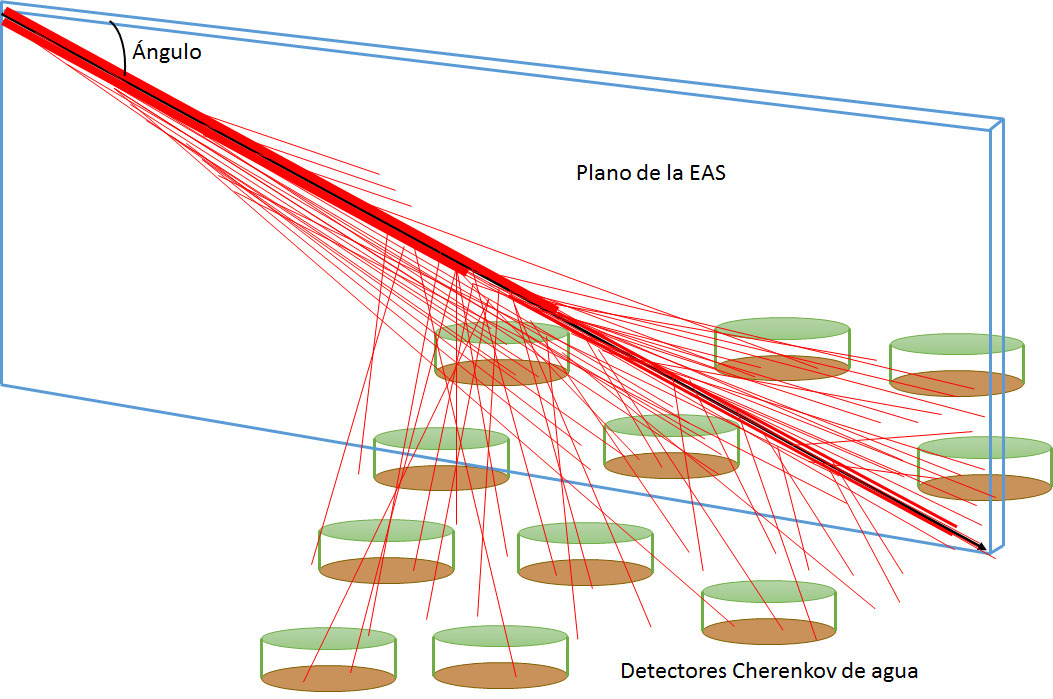
\includegraphics[width=0.8\textwidth]{Figs/imagenllu.jpeg} 
\caption[Lluvia atmósferica extendida (EAS)]
{Lluvia atmósferica extendida (EAS) detectada mediante un arreglo de varios WCD.
Procesando el tiempo con el cual el evento llega a cada detector de superficie se determina el ángulo de incidencia de las partículas ~\citep{hernandez2018procedimiento}.}
\label{lluvia}
\end{figure}

\section{Proyecto LAGO}
El proyecto LAGO (por sus siglas en inglés, \textit{The Latin American Gian Observatory}) es un observatorio de astropartículas que se dedica al estudio de temas relacionados con astrofísica y clima espacial y que cuenta con equipos instalados en diferentes países de América Latina.

\subsection{Detectores WCD de LAGO}
El proyecto LAGO utiliza tanques de agua como detectores de partículas.
Un WCD típico de LAGO es un tanque lleno de agua purificada cuyo volumen oscila entre 1~$m^3$ y 40~$m^3$.
En su interior tiene una bolsa hecha por un tejido altamente difusivo y reflectante de Tyvek~\textregistered1073D para contener todo el volumen de agua y aumentar la eficiencia de detección.
El objetivo de este recubrimiento es difundir los fotones Cherenkov captados por los tubos fotomultiplicadores (PMT, por sus siglas en inglés) y reducir la dependencia de la señal de la trayectoria de las partículas secundarias dentro del detector, ya que con esto los fotones se distribuirán uniformemente dentro del tanque (Ver Figura~\ref{tank}).

\begin{figure}[H]
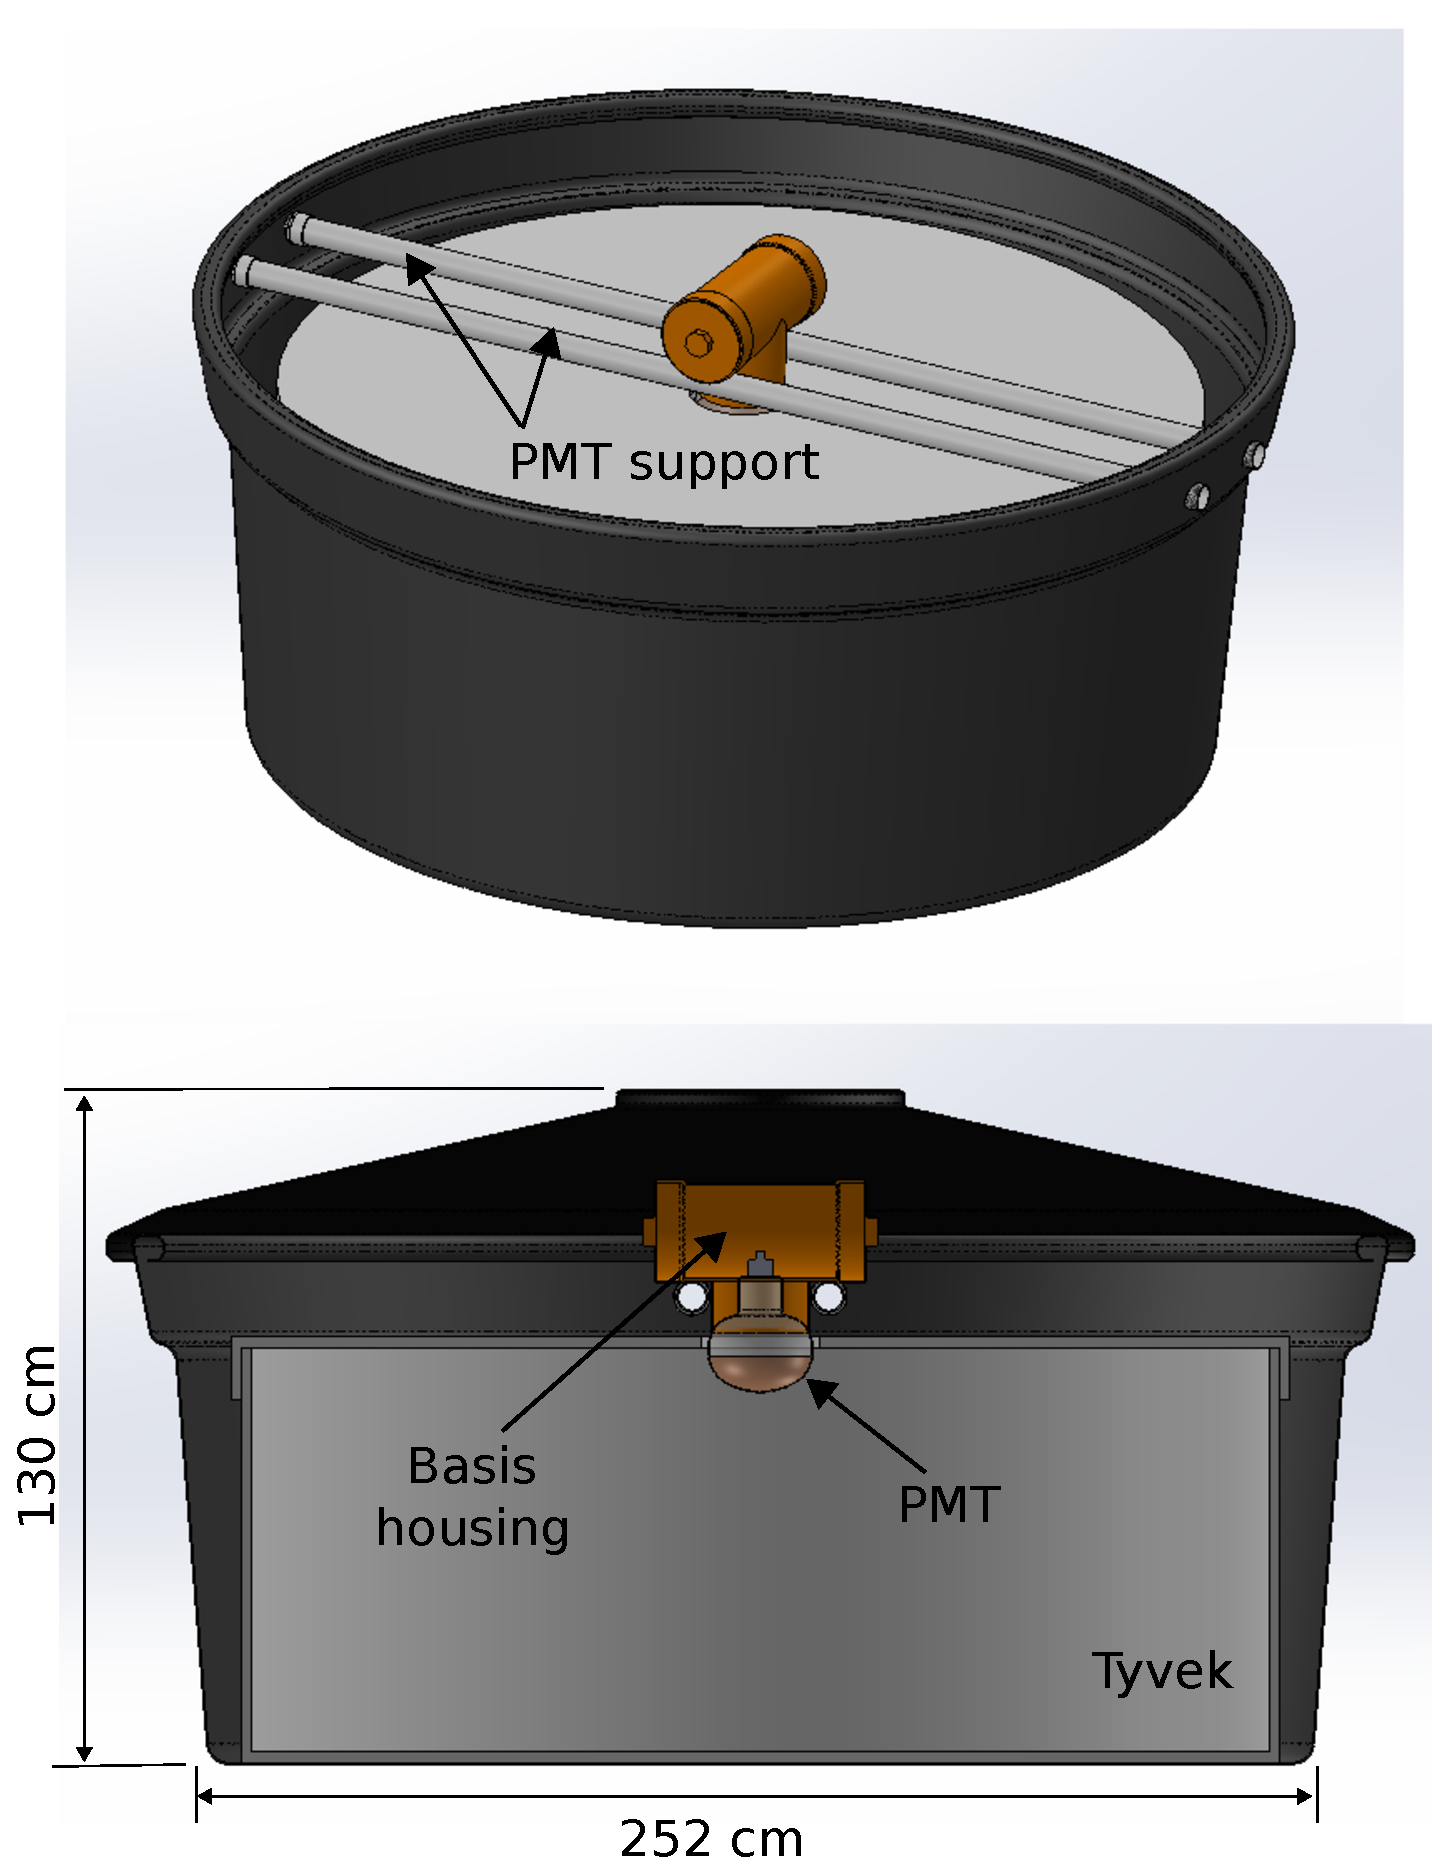
\includegraphics[scale=0.4]{Figs/Tank.eps} 
\centering
\caption[Ilustración de un Detector Cherenkov]{.~\citep{hernandez2018procedimiento}}
\label{tank}
\end{figure}

\subsection{Tubo fotomultiplicador}
Los PMT son los dispositivos fotosensores más empleados debido tanto a su gran versatilidad como sus características (respuesta rápida, alta sensibilidad y alto factor de ganancia).
Un tubo fotomultiplicador funciona como transductor y a su vez como amplificador, es decir, que a partir de una luz detectada se produce una corriente eléctrica fácilmente medible.

En la Figura~\ref{foto} se muestra el funcionamiento interno de un PMT.
Cuando los fotones de luz visible alcanzan el fotocátodo, éste emite fotoelectrones de baja energía.
Estos electrones son acelerados y multiplicados en campos eléctricos secuenciales aplicados entre los electrodos del PMT llamados dínodos.
En los dínodos la señal eléctrica es suficientemente grande para poder ser manejada con amplificadores y analizadores de pulsos convencionales.~\citep{kaptanoglu2018characterization}.


LAGO utiliza tubos fotomultiplicadores PMT Hamamatsu R5912 de 8 pulgadas desarrollados por Hamamatsu Photonics los cuales se encuentran ubicados sobre el volumen de agua donde inciden los fotones de Cherenkov. 
Estos PMT tienen 10 etapas enfocadas linealmente y su circuito de alimentación está constituido por un divisor de voltaje, una fuente de alimentación de alto voltaje y un preamplificador para acondicionar las amplitudes de los pulsos de salida.
La tensión de polarización del PMT está en el rango de 0~V a 2000~V respecto a tierra y puede controlarse con una baja tensión en el rango de 0~V a 5~V.

\begin{figure}[H]
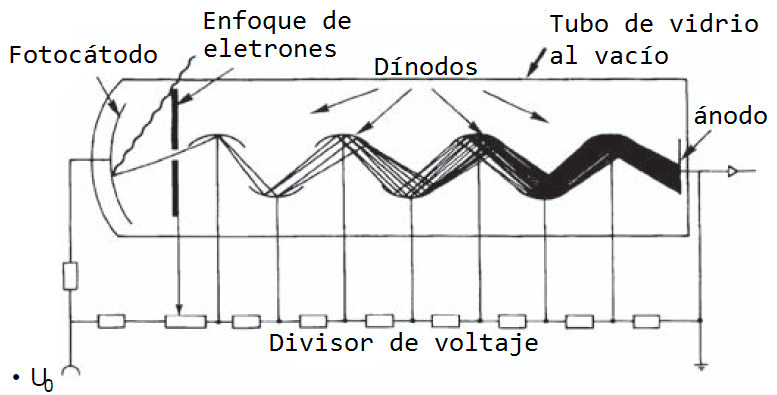
\includegraphics[scale=0.35]{Figs/pmtll.jpeg} 
\centering
\caption[Esquema de funcionamiento de un fotomultiplicador]{Esquema de funcionamiento de un fotomultiplicador.
El fotocátodo convierte la energía de luz incidente en una corriente de electrones por efecto fotoeléctrico.
El campo eléctrico creado entre los dínodos permite acelerar y guiar los electrones a lo largo del multiplicador.
El divisor de voltaje está compuesto por un arreglo de resistencias que dividen el voltaje y alimentan los dínodos.~\citep{hernandez2018procedimiento}}
\label{foto}
\end{figure}

El sistema de adquisición implementado por LAGO permite suministrar las tensiones requeridas en la base de PMT.
Un detector de WCD normalmente emite pulsos con un tiempo de subida de $\sim$10~ns y un tiempo de bajada de $\sim$70~ns.
La forma de los pulsos que vienen del detector dependen de la pureza del agua, la reflectividad del material de difusión y la geometría del tanque.~\citep{haro2016data}.
En la Figura~\ref{detec} se muestra el sistema de adquisición implementado en uno de los detectores instalado en la UIS, mientras que en la Figura~\ref{sistema_adquisicion} se muestra el diagrama de bloques de un detector WCD de LAGO.

\begin{figure}[H]
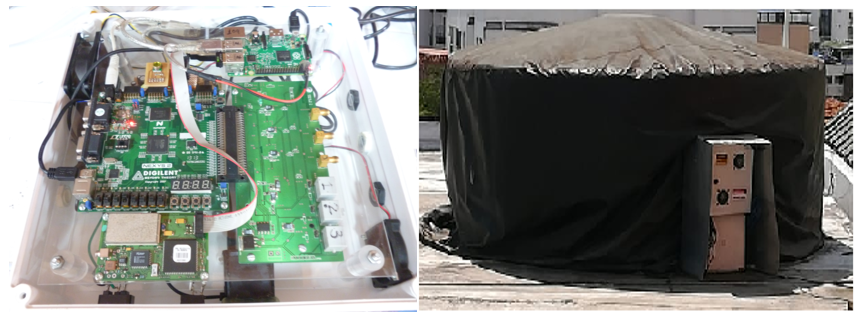
\includegraphics[scale=0.6]{Figs/lagoelectro.PNG} 
\centering
\caption[Sistema de adquisición LAGO original]{Sistema de adquisición LAGO original.
A la derecha: WCD Chitagá ubicado en el campus central de la Universidad Industrial de Santander en Bucaramanga en Santander, Colombia.
A la izquierda: electrónica del sistema de adquisición del detector.}
\label{detec}
\end{figure}

\begin{figure}[H]
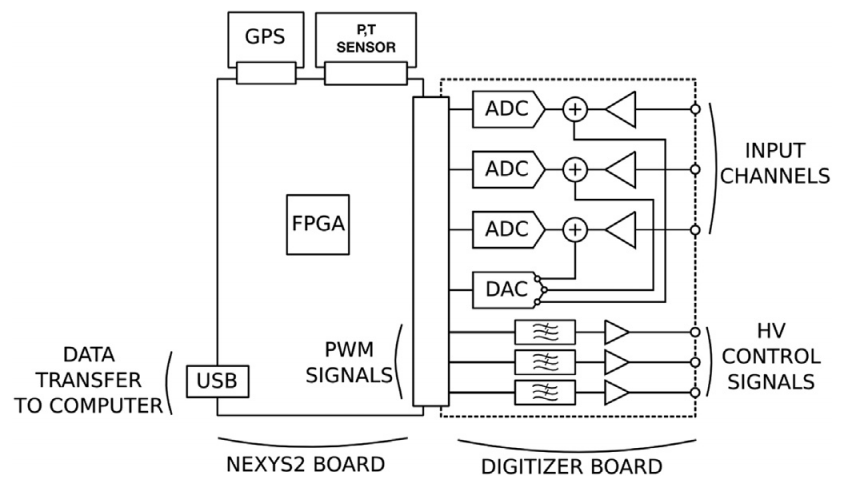
\includegraphics[scale=0.6]{Figs/bloquelago.PNG} 
\centering
\caption[Componentes principales del sistema de adquisición]{Componentes principales del sistema de adquisición: tarjeta digitalizadora de tres canales, placa Nexys-II y periféricos (GPS y sensores de temperatura y presión).~\citep{haro2016data}}.
\label{sistema_adquisicion}
\end{figure}


   % Marco teórico
% ------------------------------------------------------------------------
%                                Capítulo 3
% ------------------------------------------------------------------------
\chapter{Sistema de adquisición del proyecto LAGO}
% ------------------------------------------------------------------------
En esta sección se describe la metodología usada para alcanzar cada uno de los objetivos planteados en el plan del proyecto.
Se implementa a nivel HDL los circuitos diseñados para discriminar, digitalizar y registrar aquellos pulsos que se consideran eventos.
Además se registra la hora, geolocalización del detector, temperatura y presión atmósferica. Los datos son agrupados en un archivo de salida que se entrega para su posterior análisis.

El sistema de adquisición tiene 3 canales, para lo cual se emplea el ADC AD9235 que tiene frecuencia de muestreo máxima de 50~MHz y 12 bits de resolución.
%Esta actualización del hardware de LAGO mejora la información obtenida del evento registrado.

En la Figura~\ref{sistema} se observa el sistema de adquisición de LAGO el cual se compone de los siguientes dispositivos: 

%\begin{figure}[H]
\begin{figure}[h] % Así no queda el espacio en blanco al final de la página
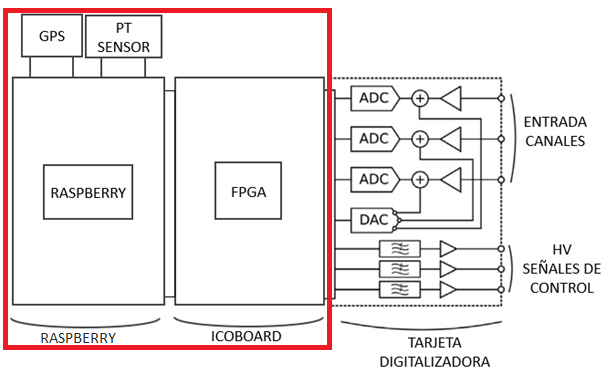
\includegraphics[scale=0.65]{Figs/pmtvie.png} 
\centering
\caption[Esquema general del sistema de adquisición actualizado]{Esquema general del sistema de adquisición actualizado, resaltando en rojo las etapas abordadas de este proyecto.} 
\label{sistema}
\end{figure}
\begin{itemize}
    \item Tarjeta electrónica que digitaliza pulsos de 3 canales independientes con salida paralela de 12 bits y una frecuencia de 50~MHz,
   \item FPGA (Icoboard) compatible con herramientas de libre desarrollo: En ella
 se implementa un conjunto de bloques jerárquicos que permiten detectar eventos relacionados con rayos cósmicos
   \item Raspberry Pi3 model B+: Permite la comunicación con los periféricos y a su vez  genera y guarda un archivo con información sobre las señales captadas y los sensores externos con el fin de establecer el tiempo de adquisición, la ubicación geográfica, la presión atmosférica y la temperatura.
   \item Dos periféricos que permitan obtener información relacionada con el entorno del WCD (ubicación, hora, temperatura ambiente y presión atmosférica.
\end{itemize}
Nota: la información proveniente de la tarjeta de digitalización será simulada con otra FPGA desde archivos existentes.\\
En la Figura~\ref{diagrama} se muestra un diagrama de bloques del sistema de adquisición implementado.
Este está compuesto por: FPGA   (Icoboard), Raspberry Pi 3   (archivo de salida), hardware externo (tarjeta de digitalización).

\begin{figure}[H]
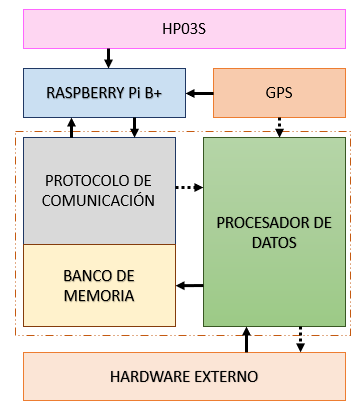
\includegraphics[scale=0.9]{Figs/hardware.PNG} 
\centering
\caption[Representación del sistema de adquisición mediante bloques]{Representación del sistema de adquisición mediante bloques. Línea discontinua: Señal de control, línea continua: Señal de control, línea discontinua naranja: FPGA.} 
\label{diagrama}
\end{figure}

%A continuación se hace una descripción funcional de cada bloque.
\section{Procesador de datos}
En la Figura~\ref{procesador} se hace una descripción funcional mediante diagrama de bloques de los circuitos de control del PMT (\texttt{RAMPA}), detección señal(\texttt{TRIGGER}), correción de línea base (\texttt{BASELINE}).

\begin{figure}[H]
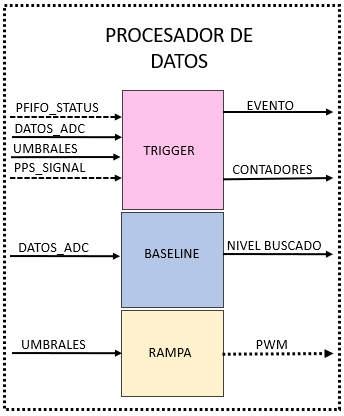
\includegraphics[scale=0.8]{Figs/procesa.PNG} 
\centering
\caption{Diagrama de bloques procesador del datos} 
\label{procesador}
\end{figure}

\subsection{Corrección de línea base}
Esta corrección se realiza con el fin de estabilizar la electrónica de adquisición frente a los efectos ambientales como la temperatura.
Es decir, si la temperatura aumenta esto provocará que la línea de base se incremente, y viceversa.
Dado que el sistema implementado compara el voltaje instantáneo en el canal ADC con una tensión de referencia (umbral de detección), cualquier cambio en el nivel de línea base podría afectar las mediciones.
Para evitar esta afectación y también el ruido electrónico se cuenta con circuitos HDL que logran mantener un valor estable de línea base en 50 niveles ADC ($\sim$49mV). 
El voltaje de línea base controlado por la FPGA se aplica a través de un convertidor de digital a analógico (DAC) de 12~bits el cual se actualiza cada 2~ms. A continuación se hace una explicación de cada uno de los bloques implementados en la FPGA para la corrección de línea base.

Para lograr una actualización de 2~ms se diseña un circuito mostrado en la Figura~\ref{actuali}  donde \textit{refresh rate} toma un valor de 100000, este valor se establece teniendo en cuenta la frecuencia del reloj de 50MHz, (período de 20 ns), entonces:
\begin{equation} \label{eq2}
     \#ciclos\times per\acute{i}odo = tiempo \rightarrow 100000 \times 20 ns = 2 ms\
\end{equation}

\begin{figure}[h]
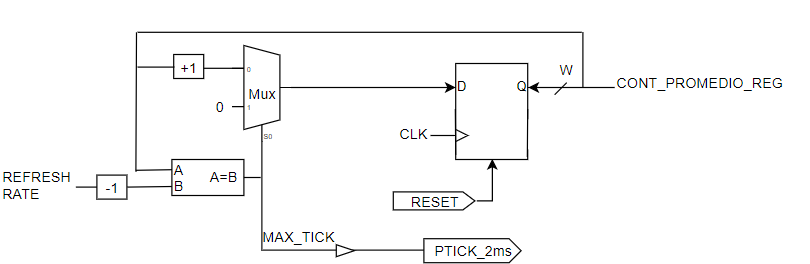
\includegraphics[width=0.9\textwidth]{Figs/CONTPROM.PNG} 
\centering
\caption{Circuito de actualización de baseline cada 2ms}
\label{actuali}
\end{figure}

El circuito de la Figura~\ref{acumulado}  muestra como los datos provenientes del ADC se acumulan durante 2~ms (MAX\_TICK) para luego hacer una comparación y lograr estabilizar la señal en $\sim$49~mV como se establece en~\citep{haro2016data}. 
El nivel de cuantización suministrado al DAC(MAX5501) se realiza en el circuito de la Figura~\ref{actu} donde se analiza la salida del acumulado (ADC\_PROM\_REG)en el contador de los ADC.

\begin{figure}[H]
\begin{minipage}[b]{0.49\linewidth}
\centering
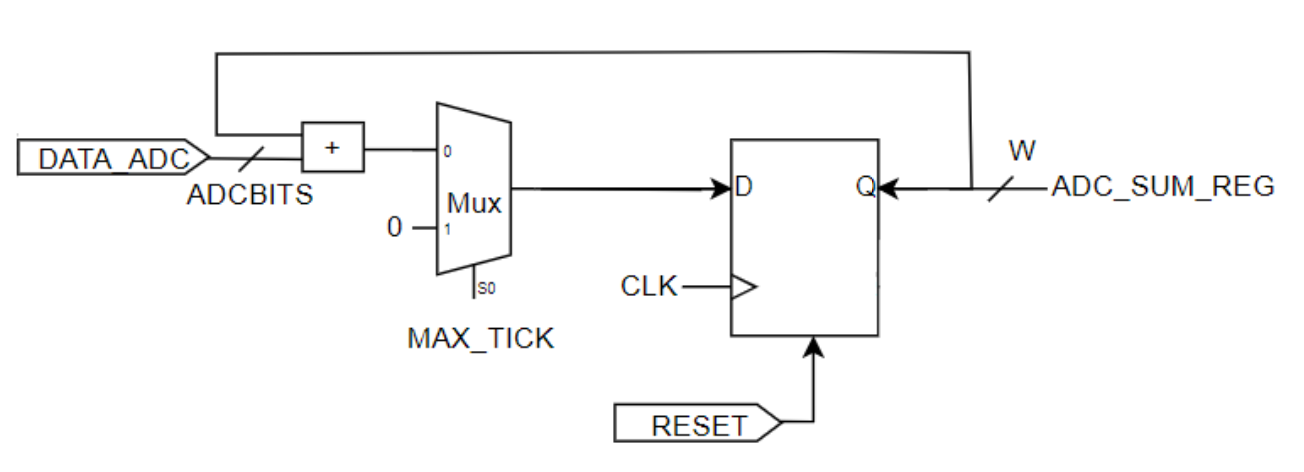
\includegraphics[width=\linewidth]{Figs/refres.PNG}
\caption{Circuito para acumular los datos provenientes de los ADC}
\label{acumulado}
\end{minipage}
\hspace{0.01cm}
\begin{minipage}[b]{0.49\linewidth}
\centering
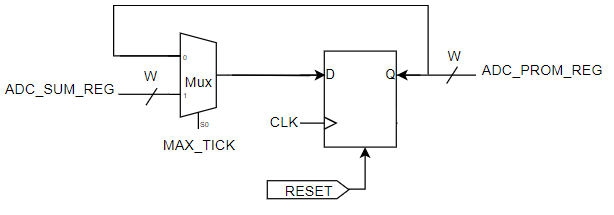
\includegraphics[width=\linewidth]{Figs/ADCPROM.PNG}
\caption{Circuito para acualizar el control de línea base cada 2~ms}
\label{actu}
\end{minipage}
\end{figure}

En ~\citep{haro2016data} se diseña un circuito inversor, cuya entrada es una señal analógica invertida. Es decir, para aumentar la salida se debe disminuir la entrada y viceversa. En el circuito Figura~\ref{salida baseline} es la señal que llega al multiplexor (MUX 2-1) y se actualiza cada 2 ms. 
Para el cálculo del módulo del circuito se tiene en cuenta los ciclos de reloj necesarios para generar 2 ms. En este caso, el nivel de voltaje buscado coincide con 50 niveles de cuantización, como se observa en la ecuación~\eqref{eq1}
\begin{equation} \label{eq1}
    \#ciclos \times nivel\_de\_cuantizaci\acute{o}n = umbral \rightarrow 100000 \times 50 = 5000000\
\end{equation}
 
\begin{figure}[h]
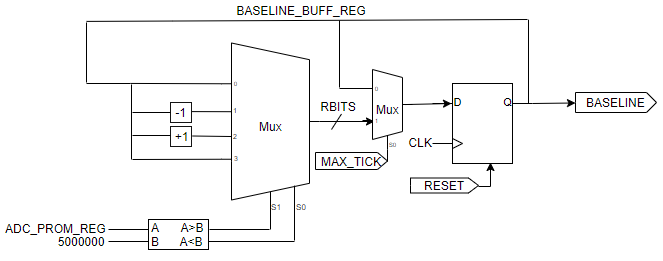
\includegraphics[scale=0.9]{Figs/base_8.PNG} 
\centering
\caption{Salida del nivel de cuantización al DAC de la línea base}
\label{salida baseline}
\end{figure}

\subsection{Regulación de  polarización de los PMT}
\label{A100}
Para el control de la fuente de alto voltaje que polariza el PMT, se genera una rampa para aumentar y/o disminuir el voltaje. 
La rampa protege los PMT de cambios bruscos de voltaje que pueden dañarlo. El usuario puede programar un set point de tensión (DATA\_IN) en el rango de 0 a 1023 en la terminal, lo que se traduce a un voltaje de 0 a 2000 V en el circuito de regulación de la fuente de polarización, como lo muestra el circuito de la Figura~\ref{registro}.

\begin{figure}[H]
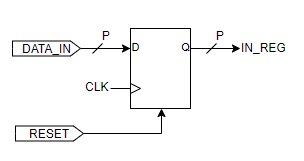
\includegraphics[scale=1]{Figs/rampa3.PNG} 
\centering
\caption{Circuito para el registro del umbral}
\label{registro}
\end{figure}

\begin{figure}[H]
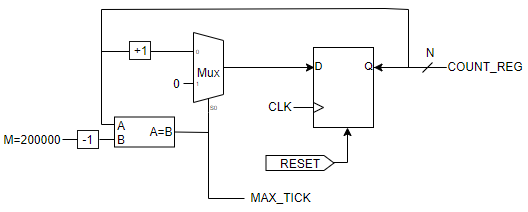
\includegraphics[scale=1]{Figs/rampa4.PNG} 
\centering
\caption{Circuito para modificar el ciclo útil de la PWM cada 2ms.}
\label{cicloutil}
\end{figure}

\begin{figure}[H]
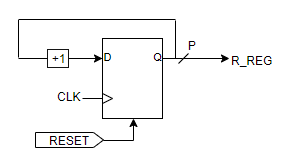
\includegraphics[scale=1]{Figs/RAMPA1.PNG} 
\centering
\caption{Circuito para generar la frecuencia de la PWM de (10~KHz)}
\label{frecuencia}
\end{figure}

El control de la PWM se establece con una frecuencia de 10~KHz Figura\ref{frecuencia} y una actualización cada 2ms Figura\ref{cicloutil} para lograr el control de su ciclo útil mediante la comparación respecto al umbral establecido por el usuario Figura~\ref{pwm}.
\begin{figure}[h]
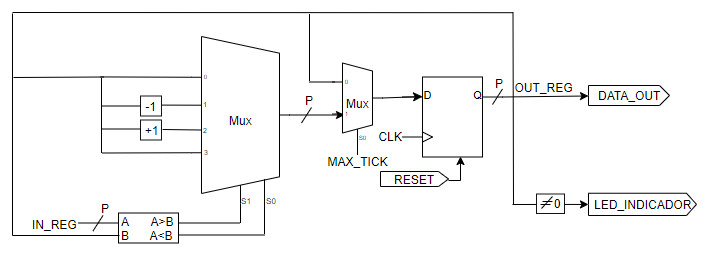
\includegraphics[width=0.9\textwidth]{Figs/RAMPA33.PNG} 
\centering
\caption[Circuito de control del ciclo útil de la PWM]{Circuito de control del ciclo útil de la PWM. (IN\_REG) es el umbral establecido por el usuario, (MAX\_TICK) actualización cada 2 ms, (OUT\_REG) es el porcentaje de ciclo útil}
\label{pwm}
\end{figure}

En el circuito de la Figura~\ref{salida} se calcula la PWM a partir de los parámetros generados anteriorimente.
(OUT\_REG) establece el porcentaje del ciclo útil y (R\_REG) la frecuencia.
De esta manera se ajusta el voltaje del PMT por medio de un conversor que interpreta la señal PWM y genera un voltaje de salida en el rango 0 a 2000V.

\begin{figure}[h]
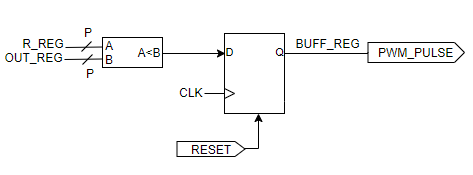
\includegraphics[scale=1]{Figs/RAMPA22.PNG} 
\centering
\caption{Circuito señal de control PWM, (OUT\_REG) ciclo útil, (R\_REG) frecuencia}
\label{salida}
\end{figure}


\subsection{Discriminación de datos (TRIGGER)}

La discriminación de los datos determina que pulsos son los que deben almacenarse. La condición Vi\textgreater Vthr determina que señal se considera un evento, donde Vi es la señal de entrada (DATA\_ADC) y Vthr es es el umbral (TRIGG\_SET). Según los análisis hechos .~\citep{haro2016data} un pulso completo se puede adquirir en una ventana de tiempo de 300 ns, garantizando que no se pierda información del evento adquirido. En este proyecto, son 15 muestras teniendo en cuenta la frecuencia de muestreo de 50~MHz.Todos los pulsos adquiridos se catalogan así: el conteo de pulsos registrados, el tiempo de ocurrencia y una etiqueta de 3 bits que identifica cual de los canales cumplió la condición de disparo.

La Figura~\ref{maquina} muestra una máquina de estados que controla todo el sistema de activación, esta permite controlar la información que se debe almacenar en orden secuencial en cada evento.

\begin{figure}[h!]
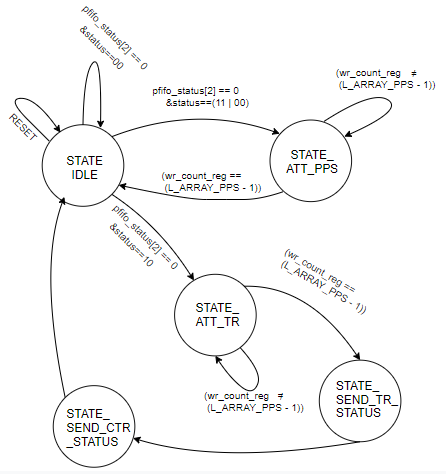
\includegraphics[width=0.8\textwidth]{Figs/fsms.PNG} 
\centering
\caption[Máquina de estados del subsistema de activación]{Máquina de estados del subsistema de activación, (STATE\_IDLE) espera, (STATE\_ATT\_PPS) reinicio de contadores cada segundo, (STATE\_ATT\_PPS) muestraeo del evento, (STATE\_SEND\_TR\_STATUS) contador del tiempo de ocurrencia del evento, (STATE\_SEND\_CTR\_STATUS) contador de eventos}
\label{maquina}
\end{figure}

El registro de desplazamiento Figura~\ref{desplazamiento} se encarga de entregar los datos provenientes de los ADC. En el registro [15] se ingresa el dato y se desplaza hasta el registro [0], esto permite hacer una comparación con el umbral de activación y  almacenar de manera simultánea la información de los 15 registros de cada canal


\begin{figure}[H]
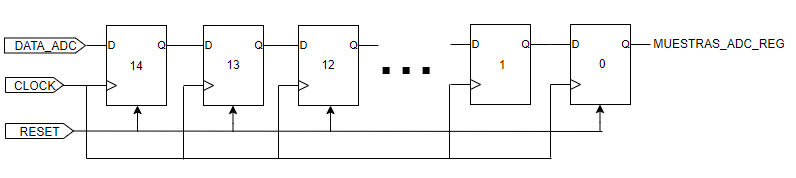
\includegraphics[width=0.9\textwidth]{Figs/registro.PNG} 
\centering
\caption{Circuito para el registro de los datos provenientes del ADC}
\label{desplazamiento}
\end{figure}

En la Figura~\ref{detectorumbral} se tiene un conjunto de comparadores conectados al registro [3, 2, 1] que determinan si el registro [3] wa mayor y los registros [2,1] son menores al umbral de activación se procede a almacenar todas las posiciones del registro anterior de la siguiente manera: se concatena la información almacenada en los registros de los 3 canales y se envía la trama resultante por comunicacion SPI de modo que pasados 15 ciclos de reloj se ha comunicado todas las muestras del evento. Ver Figura~\ref{detectorumbral}
\begin{figure}[H]
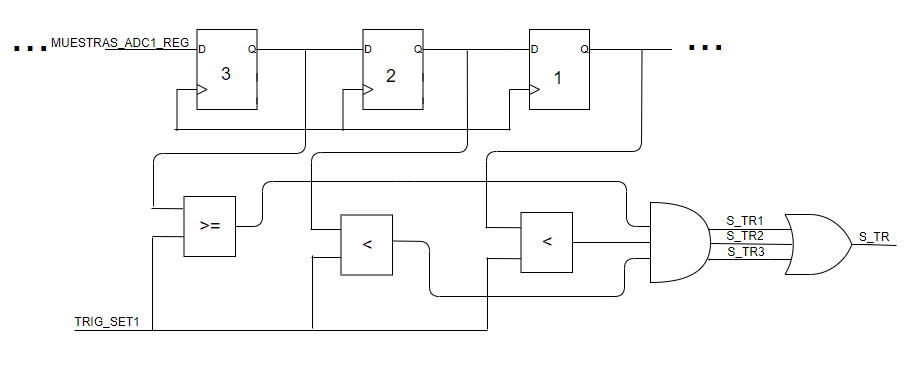
\includegraphics[width=0.9\textwidth]{Figs/COMPARA.PNG} 
\centering
\caption[Circuito de umbral de activación]{se compara la señal de entrada digitalizada(MUESTRAS$\_$ADC$\_$REG) con el umbral de activación establecido por el usuario(TRIGG$\_$SET),  si se cumple la condición de disparo se activa la señal (S$\_$TR)}
\label{detectorumbral}
\end{figure}

El circuito de la Figura~\ref{eve} concatena una bandera `10' con el contador de eventos\\ 
(CONT\_TRIGG\_REG) el cual registra el conteo de  los eventos cada vez que se cumple la condición de disparo en alguno de los 3~canales. 

\begin{figure}[h!]
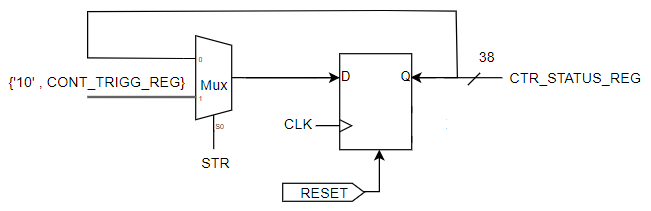
\includegraphics[scale=0.9]{Figs/ctr_status.PNG} 
\centering
\caption[Circuito concatenación trama de datos a comunicar protocolo SPI]{Circuito concatenación trama de datos a comunicar (CTR$\_$STATUS$\_$REG), (S$\_$TR) habilitador  del disparo, (CONT$\_$TRIGG$\_$REG) contador de eventos}
\label{eve}
\end{figure}

En la Figura~\ref{flancos}, el circuito se activa cada vez que se cumple la condición de disparo. Este registra el tiempo de ocurrencia, y asigna una máscara de 3 bits [S\_TR3, S\_TR2, S\_TR1] para detectar cual canal se dispara .

\begin{figure}[H]
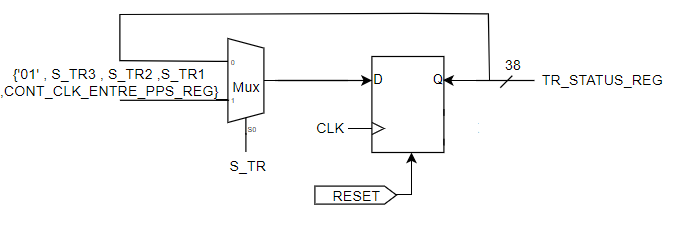
\includegraphics[scale=0.9]{Figs/tr_status.PNG} 
\centering
\caption[Circuito concatenación trama de datos a comunicar protocolo SPI ]{Circuito de concatenación de la trama de los datos a comunicar (TR$\_$STATUS$\_$REG), etiquetas de activación para cada canal (S$\_$TR3,S$\_$TR2,S$\_$TR1), contador tiempo entre cada evento (CONT$\_$CLK$\_$ENTRE$\_$PPS$\_$REG)}
\label{flancos}
\end{figure}

Para controlar el reinicio sincronizado de los contadores de tiempo de ocurrencia se diseña la siguiente máquina de estados que dispone de la señal pulso por segundo (PPS) la cual proviene del GPS. Ver Figura~\ref{pps}
\begin{figure}[h!]
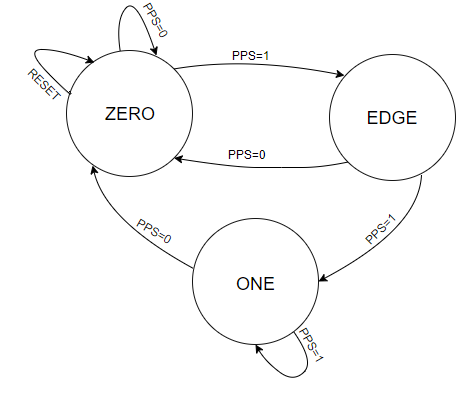
\includegraphics[scale=0.8]{Figs/MAQUINA1.PNG} 
\centering
\caption[Máquina de estados del conteo de pulsos por segundo]{Máquina de estados del conteo de pulsos por segundo, (ZERO) estado de reposo, (PPS) señal del GPS que permite activar el estado (EDGE) y por consiguiente el estado (ONE)}
\label{pps}
\end{figure}

En caso de no disponer de GPS, un circuito auxiliar divisor de frecuencia a 1 Hz se encarga de contar los flancos ascendentes del clk de la FPGA para simular la señal PPS y generar un PPS\_FALSO, con el fin de no afectar la adquisición de los eventos. Ver Figura~\ref{ppsfalso} 

\begin{figure}[H]
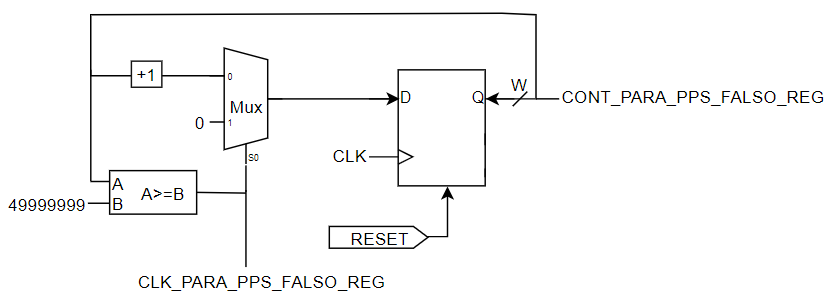
\includegraphics[width=0.9\textwidth]{Figs/CONPPSFALSO.PNG} 
\centering
\caption{Circuito de generación del PPS$\_$FALSO}
\label{ppsfalso}
\end{figure}

El circuito de la Figura~\ref{comparafalso} modula el ciclo útil del PPS\_FALSO a 100 ms.

\begin{figure}[H]
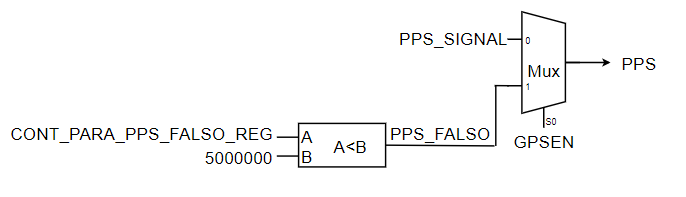
\includegraphics[scale=0.8]{Figs/PPSP.PNG} 
\centering
\caption[Circuito para generar la señal PPS]{Circuito para generar la señal PPS, selecciona la señal proveniente del GPS (PPS$\_$SIGNAL) o una señal simulada (PPS$\_$FALSO), en caso de ausencia del GPS (GPSEN)}
\label{comparafalso}
\end{figure}

Si se activa el PPS\_FALSO se activa un led de indicación se muestra en la Figura~\ref{ledfalso}
\begin{figure}[H]
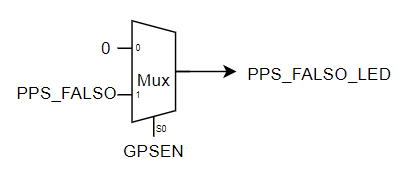
\includegraphics[scale=0.8]{Figs/TRIGER5.PNG} 
\centering
\caption{Circuito de activación de PPS\_FALSO\_LED}
\label{ledfalso}
\end{figure}

\section{\textbf{Protocolo de comunicación}}
Este bloque logra la comunicación entre la FPGA y la Raspberry para la transmisión y recepción de la información; el protocolo se basa en el estándar SPI, donde la Raspberry es el maestro y la FPGA el esclavo. Este protocolo fue elegido teniendo en cuenta que la tasa de detección de un WCD típico en LAGO puede alcanzar valores hasta de 2 KHz.~\citep{hernandez2018procedimiento}

\begin{figure}[H]
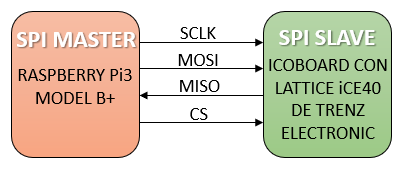
\includegraphics[scale=1]{Figs/SPIPROTO.PNG} 
\centering
\caption[Esquema protocolo SPI]{Protocolo SPI se compone de 4 señales así: SCLK señal de reloj proviniente del maestro Raspberry Pi 3, MOSI señal que permite llevar los bits del maestro hacia el esclavo, MISO señal que permite llevar los bits del esclavo al maestro y CS señal que se encarga de habilitar el esclavo} 
\label{adecuacion}
\end{figure}

El protocolo SPI utilizado en el proyecto fue basado en .~\citep{charkster/spi_slave_verilog_2020} en el cual se implementa un  SPI Slave y un mapa de memoria diseñado para la comunicación entre una FPGA y una Raspberry. En la Figura~\ref{spi} se muestra el RTL(Register-transfer-level) del protocolo implementado.

\begin{figure}[H]
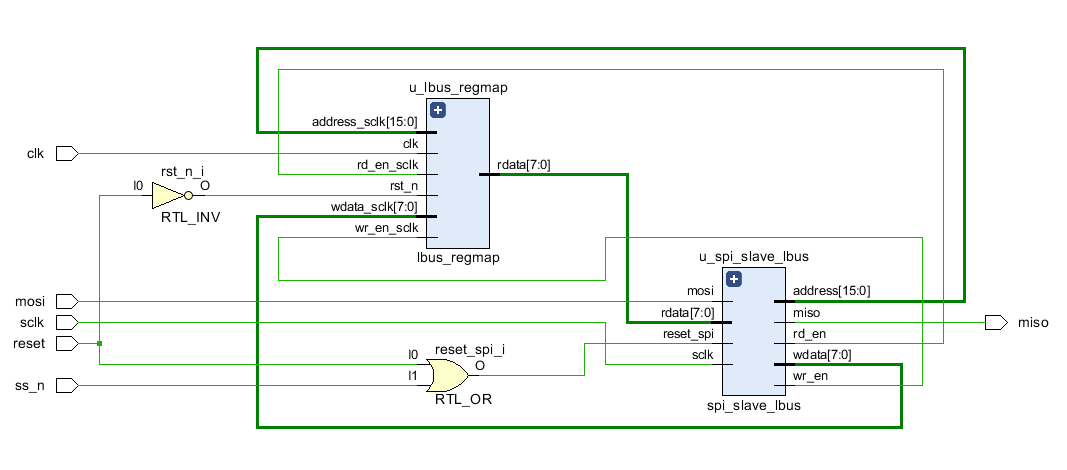
\includegraphics[width=0.93\textwidth]{Figs/rtlproto.PNG} 
\centering
\caption{RTL protocolo de comunicación SPI .~\citep{XilinxInc.2016IntegratedGuide}} 
\label{spi}
\end{figure}

El mapa de memoria del protocolo se modifica y redimensiona para almacenar los eventos provenientes de los ADC.
La Tabla~\ref{tab:my-table} muestra como se ha distribuido los datos transferidos y la posición de memoria asignada para cada uno, obteniendo una totalidad de 98 posiciones con un ancho de 8 bits para cada una.

\begin{table}[h!]
\centering
\begin{tabular}{|c|c|c|c|c|}
%\hline
%\multicolumn{5}{|c|}{\cellcolor[HTML]{E0E0E0} MAPA DE MEMORIA PROTOCOLO SPI }\\
\hline
%\multicolumn{2}{|c|}{Posición} &  & \multicolumn{1}{l|}{}&\\
Posición & Posición      & & Bits & \\ 
Inicial & Final         & \multirow{-2}{*}{Dato} & usados & \multirow{-2}{*}{Descripción}\\
\hline
 0 &  1 & Trigger 1     & 12 & \\ \cline{1-4}
 2 &  3 & Trigger 2     & 12 & \\ \cline{1-4}
 4 &  5 & Trigger 3     & 12 & \\ \cline{1-4}
 6 &  7 & Rampa 1       & 12 & \\ \cline{1-4}
 8 &  9 & Rampa 2       & 12 & \\ \cline{1-4}
10 & 11 & Rampa 3       & 12 & \multirow{-6}{*}{\begin{tabular}[c]{@{}c@{}}Parámetros\\
                                ingresados\\ por usuario\end{tabular}} \\ \hline
12 & 12 & Pfifo\_status & 1  & Señal de control \\ \hline
13 & 17 & Muestra 1     & 38 & \\ \cline{1-4}
18 & 22 & Muestra 2     & 38 & \\ \cline{1-4}
23 & 27 & Muestra 3     & 38 & \\ \cline{1-4}
28 & 32 & Muestra 4     & 38 & \\ \cline{1-4}
33 & 37 & Muestra 5     & 38 & \\ \cline{1-4}
38 & 42 & Muestra 6     & 38 & \\ \cline{1-4}
43 & 47 & Muestra 7     & 38 & \\ \cline{1-4}
48 & 52 & Muestra 8     & 38 & \\ \cline{1-4}
53 & 57 & Muestra 9     & 38 & \\ \cline{1-4}
58 & 62 & Muestra 10    & 38 & \\ \cline{1-4}
63 & 67 & Muestra 11    & 38 & \\ \cline{1-4}
68 & 72 & Muestra 12    & 38 & \\ \cline{1-4}
73 & 77 & Muestra 13    & 38 & \\ \cline{1-4}
78 & 82 & Muestra 14    & 38 & \\ \cline{1-4}
83 & 87 & Muestra 15    & 38 & \\ \cline{1-4}
88 & 92 & Contador 1    & 38 & \\ \cline{1-4}
93 & 97 & Contador 2    & 38 & \multirow{-17}{*}{\begin{tabular}[c]{@{}c@{}}Trama\\ de datos\\ evento\end{tabular}}  \\
\hline
\end{tabular}
\caption{Mapa de memoria protocolo SPI}
\label{tab:my-table}
\end{table}

%\newpage
\section{\textbf{Hardware externo de emulación}}

Teniendo en cuenta que este proyecto se compone sólo de la parte digital del sistema DAQ de LAGO. Los datos de eventos que pueden ser considerados rayos cósmicos fueron simulados desde un archivo de salida ya existente. Estos fueron almacenados en las memorias ROOM de una FPGA Nexys 4-DDR (nombrada de ahora en adelante solo Hardware externo) para simular el ADC en condiciones de detección.
Con esta estrategia se consigue simular la electrónica de digitalización.

El Hardware externo recibe una señal de reloj a 50MHz proveniente de la FPGA Icoboard para sincronizar la de información almacenada en las memorias. 
 
\begin{figure}[h]
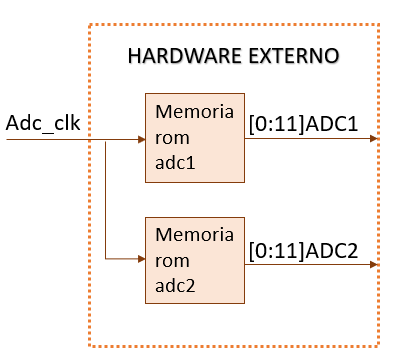
\includegraphics[scale=0.7]{Figs/hardexter.PNG} 
\centering
\caption[Diagrama de bloques hardware externo]{Diagrama de bloques hardware externo, Adc\_clk es la señal de reloj transmitida por la Icoboard}
\label{adecuacion}
\end{figure}
Ha sido necesario incluir una descripción  que permite sincronizar en frecuencia y fase los relojes de las dos FGPA y así asegurar que las muestras se entreguen sin pérdida de información por violación de tiempos.

\section{Raspberry pi 3 B+}

\begin{figure}[H]
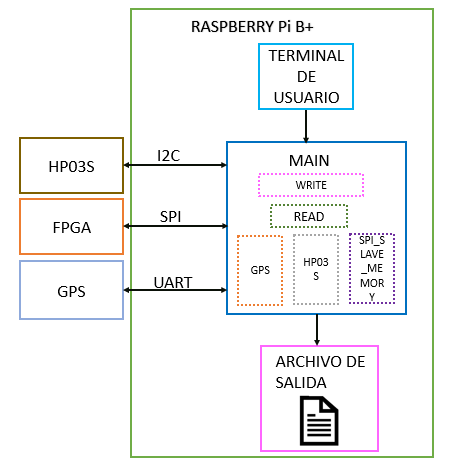
\includegraphics[scale=0.8]{Figs/raspidiagrama.PNG} 
\centering
\caption{Diagrama de bloques Raspberry Pi}
\label{rasp}
\end{figure}

La Raspberry almacena las tramas de datos que componen un evento y registra los datos obtenidos de tres dispositivos que conforman el sistema de adquisición a través de diferentes protocolos de comunicación como se muestra en la Figura~\ref{rasp}.
\begin{itemize}
    \item Protocolo SPI para la FPGA Icoboard: permitiendo acceder a los registros para configurar parámetros de adquisición y envío de los eventos registrados. 
    \item Protocolo I2C para el sensor HP03S: por medio de la librería wiringPiI2C se configura la comunicación según. ~\citep{HP03SDatasheet}.
    \item Protocolo UART con sensor GPS: se obtiene lectura hora y  geoposicionamiento según. ~\citep{Adafruit2020}.

\end{itemize}


%La comunicación con el sensor HP03S se logra con I2C según la   hoja de datos ~\citep{HP03SDatasheet},importando librerías al    software como <wiringPiI2C>.
 
%La comunicación con el GPS se realiza a través del protocolo UART para lograr la lectura y escritura de los datos de hora y geoposicionamiento al software ~\citep{Adafruit2020}.

Finalmente el archivo \texttt{Main} corresponde a un \textit{script} en Python donde se establece el llamado de todas las funciones, recopilando toda la información.
Además, se crea una interfaz de usuario para el ingreso de parámetros por medio de una terminal.
Posteriormente se entrega un archivo de salida que presenta el registro de los eventos.





%----------------------------------------------------------------------------------------------------------------   % sistema de adquisición proyecto LAGO
% ------------------------------------------------------------------------
%                                Capítulo 4
% ------------------------------------------------------------------------
\chapter{Implementación proyecto LAGO}
% ------------------------------------------------------------------------.
\section{FPGA}

\begin{figure}[h]
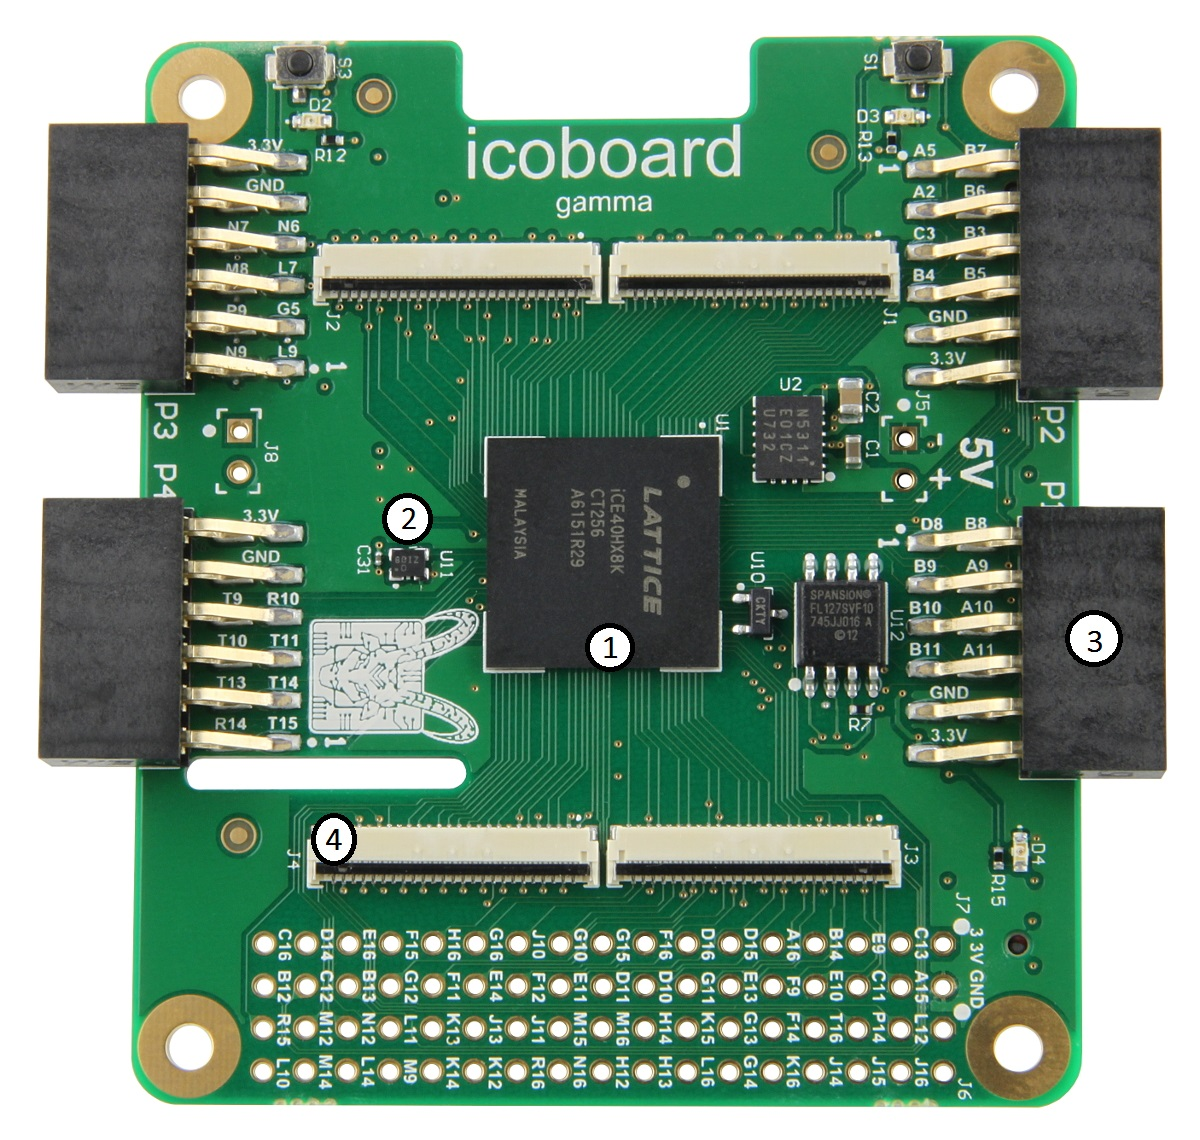
\includegraphics[scale=0.18]{Figs/icoboard.jpg} 
\centering
\caption{Icoboard con Lattice iCE40 de Trenz Electronic con SRAM de 8 MBit.~\citep{IcoBoard}}
\label{icoboard}
\end{figure}

En este trabajo se selecciona la placa ICOBOARD que se muestra en la Figura~\ref{icoboard},  contiene una FPGA Lattice con 8K LUT (1), un reloj de 100 MHz (2), 8 MBit de SRAM programable en Verilog por una cadena de herramientas de código abierto, 4 conectores Pmod de 16 entradas y salidas (E/S) (3) Y 4 conectores Flat flex cada uno con 36 E/S (4). Es responsable del pre-procesamiento de los datos, el ajuste de umbrales de activación, el ajuste de los voltajes de compensación de línea base y regulación de la fuente de alto voltaje para los PMT.



%A continuación se muestra en la Figura~\ref{herramientas}la cadena de herramientas utilizadas para una descripción de sistemas digitales sintetizables en FPGAs usando sólo herramientas libres y una descripción del hardware en lenguaje Verilog.
 
%\begin{figure}[H]
%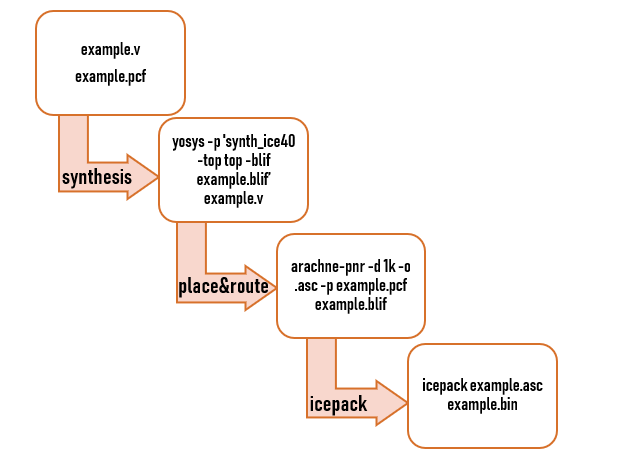
\includegraphics[scale=0.68]{Figs/progra.PNG} 
%\centering
%\caption{Cadena de herramientas para cargar archivos en icoboard}
%\label{herramientas}
%\end{figure}

La Icoboard es compatible con la Raspberry, es por medio de esta que se carga el archivo ejecutable en la FPGA. La Figura~\ref{Compatilidad} muestra un diagrama de bloques para la comunicación entre las dos tarjetas. 

\begin{figure}[h]
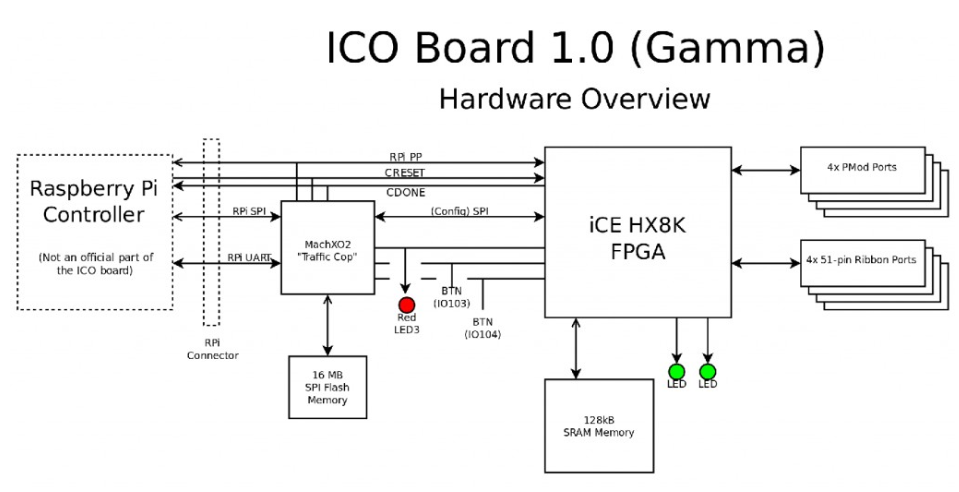
\includegraphics[width=0.93\textwidth]{Figs/icogama.PNG} 
\centering
\caption{Compatibilidad con la raspberry~\citep{IcoBoard}}
\label{Compatilidad}
\end{figure}

%\begin{itemize}
%    \item Recursos de la FPGA seleccionada
%\end{itemize}

%Nótese en la figura anterior el LCMXO2-256HC-4SG32I este el sistema embebido  FPGAs (Field Programmable Gate Array) de la Icoboard, cuenta con una memoria flash SPI de 16MB.

A continuación se describe de manera detallada los recursos lógicos disponibles en la FPGA Icoboard.

La Figura~\ref{arquitectura}  muestra la arquitectura programable. La Icoboard tiene la disponibilidad de 4 bancos de puertos I/O los cuales son necesarios para la adquisición en paralelo de los 3 canales con una resolución de 12 bits, demandando una totalidad de 36 entradas. %sólo para adquirir la información de los 3 canales. 


\begin{figure}[H]
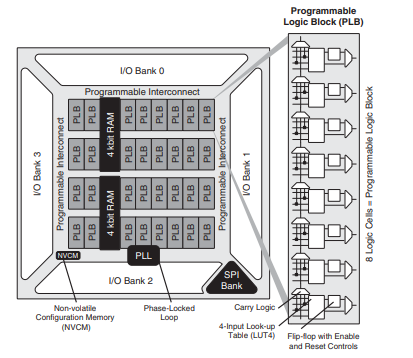
\includegraphics[scale=1.2]{Figs/architecture.PNG} 
\centering
\caption{Arquitectura iCE40~\citep{LatticeSemiconductor2017}}
\label{arquitectura}
\end{figure}

\noindent En la Figura~\ref{adecuacion2} se muestran los recursos lógicos disponibles para la implementación de la descripción en hardware.
Según los reportes de utilización que entrega el software utilizado Arachne, la implementación del proyecto necesita:
\begin{itemize}
    \item 38 entradas/salidas
    \item Celdas lógicas utilizadas:4335
    \item Flip Flop tipo D: 2435
\end{itemize}
Con esto se determina que la descripción en hardware necesario puede ser soportado por la FPGA seleccionada.

\begin{figure}[H]
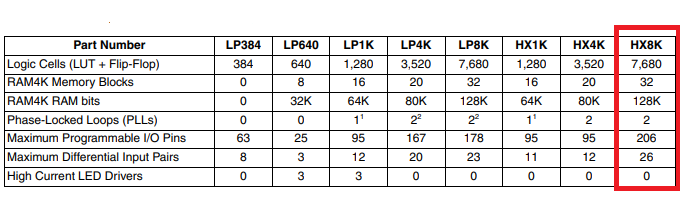
\includegraphics[width=0.93\textwidth]{Figs/tabla.png} 
\centering
\caption{Recursos lógicos de la FPGA Icoboard~\citep{LatticeSemiconductor2017}}
\label{adecuacion2}
\end{figure}


\section{Sensores adicionales}
En esta sección se describen los sensores usados para el proyecto, los cuales son de vital importancia para los análisis posterior del archivo de salida. El sensor de temperatura y presión barométrica permite conocer las condiciones atmósfericas básicas bajo las cuales trabaja el WCD, y de esta manera, se obtiene información de las variaciones de temperatura que afectan el comportamiento del detector y por tanto generar alteraciones en la tasa de eventos registrados.

Por otra parte, el GPS seleccionado (Adafruit Ultimate) permite conocer las condiciones de geoposicionamiento del detector, además permite la sincronización temporal de la interfaz digital al usar la señal PPS (Pulse-Per-Second).

A continuación se muestra las características más relevantes de los sensores usados.

\subsection{GPS}
Un criterio importante para la configuración entre Raspberry-GPS-FPGA es la necesidad de generar un archivo de salida de datos como se planteo en los objetivos que contenga una referencia temporal precisa, para relizar estudios dinámicos.
También, la información de geoposicionamiento del flujo de rayos cósmicos secudarios es un factor relevante que afecta el flujo de partículas detectadas con parámetros como la altura a nivel del mar y la latitud.

Es importante que el GPS seleccionado tenga la señal PPS (Pulse-Per-Second) como uno de sus periféricos. 
Esta señal y el tiempo UTC del GPS proporcionan la información de tiempo a la Raspberry Pi.

Dentro las características más relevantes del GPS está el periférico PPS, Y una interfaz de comunicación UART a 9600 baud.

%Vin range: 3.0-5.5VDC, Velocidad de adquisición: 0.1 m/s.
%___________________________Seguir revisando

\begin{figure}[H]
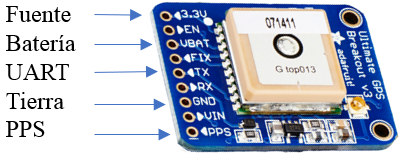
\includegraphics[scale=0.85]{Figs/gps.png} 
\centering
\caption{GPS adafruit ultimate~\citep{Adafruit2020}}
\label{adecuacion}
\end{figure}

\subsection{Temperatura y presión atmosférica}
El sensor de temperatura y presión utilizado cuenta con una interfaz de comunicación I2C, un convertidor análogo digital con 16 bits de resolución que proporciona datos de la presión y la temperatura. 
El sensor es calibrado por el fabricante almacenando 11 coeficientes únicos en el chip, los cuales se usan en la lectura de presión y temperatura. 
Este dispositivo opera con 3V, una corriente de 500uA durante la conversión y 1uA en reposo.

\begin{figure}[H]
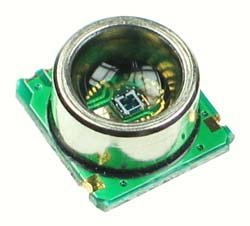
\includegraphics[scale=0.7]{Figs/hp03s.jpg} 
\centering
\caption{Sensor HP03S de presión y temperatura ~\citep{HP03SDatasheet}}
\label{adecuacion}
\end{figure}

\begin{figure}[H]
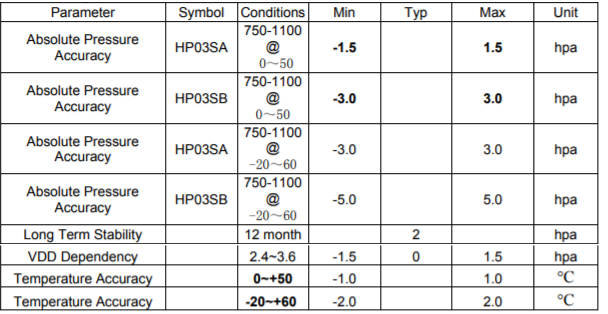
\includegraphics[width=0.93\textwidth]{Figs/tabla_hp03s.PNG} 
\centering
\caption{Caracteristicas de salida del sensor de presión y temperatura ~\citep{HP03SDatasheet}}
\label{adecuacion}
\end{figure}



\section{Raspberry Pi B+}
Se eligió la Raspberry Pi3 Model B+ puesto que esta cumple con los requerimientos necesarios para el desarrollo del proyecto.
%y además existían unidades en el grupo Halley.

\begin{table}[h] 
\begin{center}
\begin{tabular}{|p{4cm}|p{10cm}|}\hline
%\rowcolor[HTML]{FFFFC7} 
%\multicolumn{2}{|c|} {RASPBERRY PI 3 MODEL B+}\\ \hline  
\textbf{Procesador} & Broadcom BCM2837B0, Cortex-A53 (ARMv8) 64-bit SoC\\ \hline
\textbf{Frecuencia de reloj}& 1,4 GHz\\ \hline
\textbf{Memoria}    & 1GB LPDDR2 SDRAM\\ \hline
\textbf{Conectividad inalámbrica} & 2.4GHz / 5GHz IEEE 802.11.b/g/n/ac Bluetooth 4.2, BLE\\ \hline
\textbf{Conectividad de red} & Gigabit Ethernet over USB 2.0 (300 Mbps de máximo teórico)\\ \hline 
\textbf{Puertos}    & GPIO 40 pines, HDMI, 4 x USB 2.0, CSI (cámara Raspberry Pi), DSI (pantalla tácil), Toma auriculares / vídeo compuesto, Micro SD, Micro USB (alimentación), Power-over-Ethernet (PoE)\\ \hline
\end{tabular}
\caption{Características Raspberry Pi3 Model B+~\citep{Pasor2018}}
\label{tabla2}
\end{center}
\end{table}

Sus características más destacadas se muestran en la Tabla~\ref{tabla2}. Tiene una frecuencia de 1,4 GHz para sus cuatro núcleos  ayudando a obtener mejores rendimientos en muchas de las tareas que se propongan a este miniPC. 
La plataforma soporta diversos sistemas operativos, desde GNU/Linux hasta algunas versiones de Windows, para el caso del proyecto se utiliza Raspian (distribución de GNU/Linux basado en Debian para Raspberry PI).

Uno de los retos que se presentan en el desarrollo del proyecto es adquirir los datos de interés y almacenarlos, por esta razón se utilizaron librerías que permiten el uso de pines GPIO (General Purpose Input Output) con el lenguaje de medio nivel (C o C++) y Python, esto con el fin de hacer uso eficiente de los recursos del sistema.
%, de tal manera que el procesador no se ocupe en procesos innecesarios.


\section{Integración de periféricos}
Este circuito se implementa para tener la conexión de la Raspberry y la FPGA con los periféricos de una manera más organizada y así lograr la comunicación de todos los componentes utilizados en el proyecto.

La PCB se diseña a doble capa, esta es compatible con una amplia gama de Raspberry y tiene dimensiones de 56.4 x 65.9 mm.
Ver Figura~\ref{pcb}.

\begin{figure}[H]
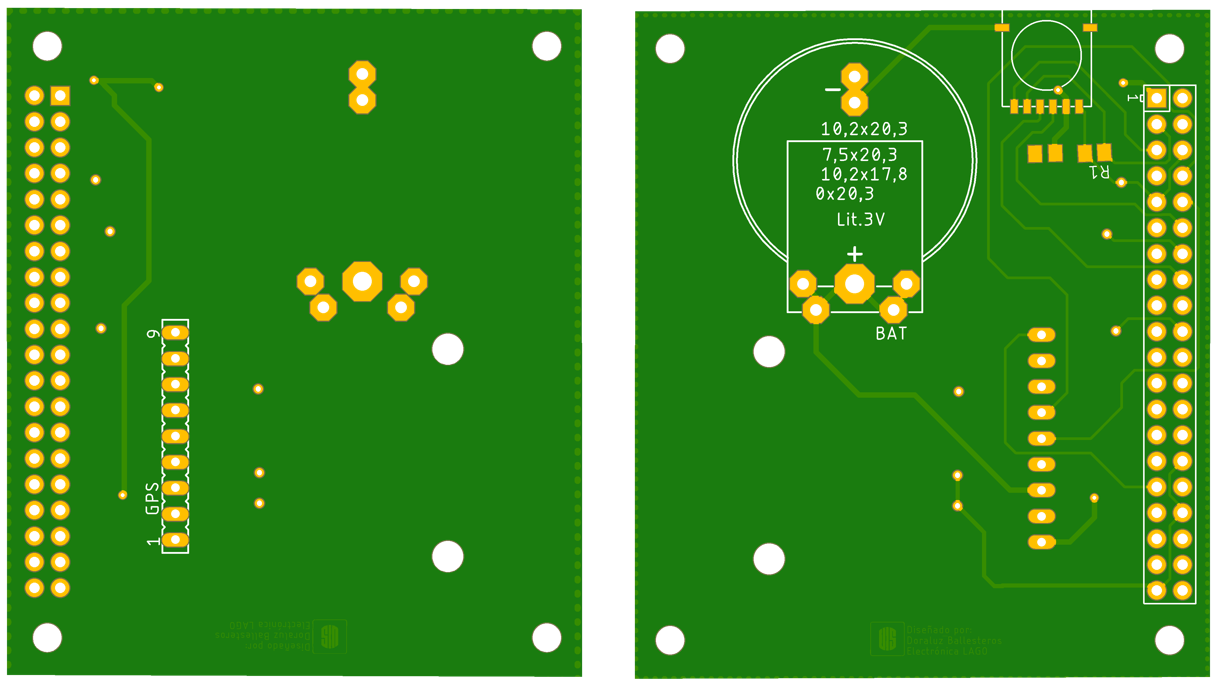
\includegraphics[width=0.90\textwidth]{Figs/pcb_eagle.PNG} 
\centering
\caption{Diseño de la PCB}
\label{pcb}
\end{figure}

En la Figura~\ref{pcb} se muestra una tarjeta ''shield'' donde se realiza la comunicación teniendo en cuenta cada uno de los protocolos que permiten recibir la información suministrada por los sensores.
En la PCB diseñada se realizaron conexiones del protocolo UART para el GPS Adafruit Ultimate e I2C para el sensor de presión y temperatura HP03S con pines de la Raspberry pi3 B+. 

\begin{figure}[H]
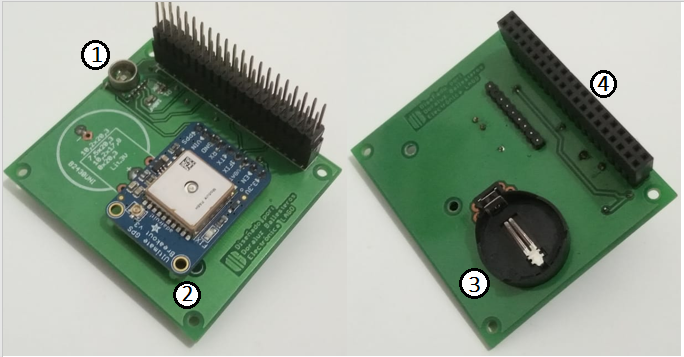
\includegraphics[width=0.85\textwidth]{Figs/pcb.PNG} 
\centering
\caption{PCB de integración de periféricos}
\label{pcb}
\end{figure}

Se integran los perifericos captadores así: sensor HP03S (1), GPS Adafruit Ultimate (2), batería (3), conector 40 pines (4).

\begin{figure}[H]
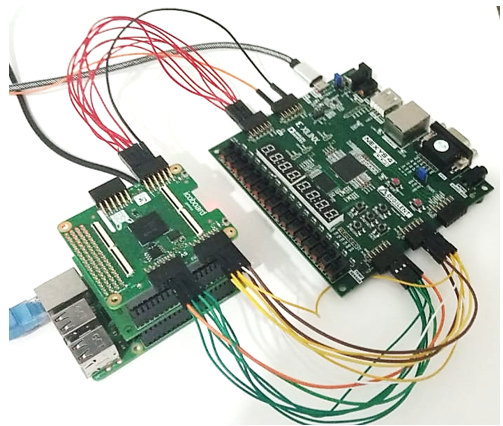
\includegraphics[scale=0.75]{Figs/lagofinal.PNG} 
\centering
\caption{Implementación proyecto LAGO para pruebas con nexys 4-DDR}
\label{nexys}
\end{figure}
En la Figura~\ref{nexys} se puede observar la conexión implementada para simular la señales provinietes de la targeta digitalizadora presentada en la Figura~\ref{sistema}  por medio de una Nexys 4-DDR.


\begin{figure}[H]
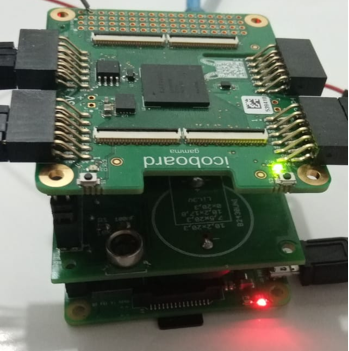
\includegraphics[scale=0.85]{Figs/icoboardfinal.PNG}
\centering
\caption{Implementación del hardware LAGO actualizado}
\label{lagofin}
\end{figure}

En la Figura~\ref{lagofin} se encuentra ubicado de abajo hacia arriba la Raspberry PI model B+, PCB con perifericos y la FPGA Icoboard.

Note que la Raspberry alimenta a todo el cojunto de tarjetas, esta entrega una tensión de 3,3 V.

%\begin{figure}[H]
%\includegraphics[scale=0.2]{Figs/P1070196.JPG} 
%\centering
%\caption{Implementación proyecto LAGO original }
%\label{original}
%\end{figure}

%Finalmente se implementa e
El diseño final del sistema de adquisición se muestra en la Figura~\ref{lagofin}, nótese que se ve mucho más compacto  que el LAGO original Figura~\ref{adecuacion}, excepto por nexys 4-DDR usada como hardware externo para las pruebas Figura~\ref{nexys}.

% ------------------------------------------------------------------------   % implementación proyecto LAGO
% ------------------------------------------------------------------------
% ------------------------------------------------------------------------
% ------------------------------------------------------------------------
%                            Recomendaciones
% ------------------------------------------------------------------------
% ------------------------------------------------------------------------
% ------------------------------------------------------------------------

\chapter{Resultados}

En esta sección se evidencia en primera instancia las simulaciones a nivel RTL de los circuitos descritos en HDL para la actualización del proyecto LAGO. A su vez  los resultados se comparan con las mediciones del hardware en el proyecto original evidenciando la respuesta del sistema ante una entrada conocida.

Para verificar el diseño de los circuitos descritos a nivel RTL en la FPGA se toma un archivo de los ya existentes de LAGO y se ingresa mediante memorias en la FPGA de emulación en este caso la Nexys 4 para entregar los datos provenientes del ADC y esta se conecta  la FPGA Icoboard para hacer todo el procesamiento de los datos provenientes de los adc y así determinar los eventos para finalmente en la Raspberry se guarda la infomacion junto con los datos provenientes de los periféricos para entregar todo complilado en el archivo de salida .dat. Esta verificación se muestra en la Figura~\ref{verifi}.

\begin{figure}[H]
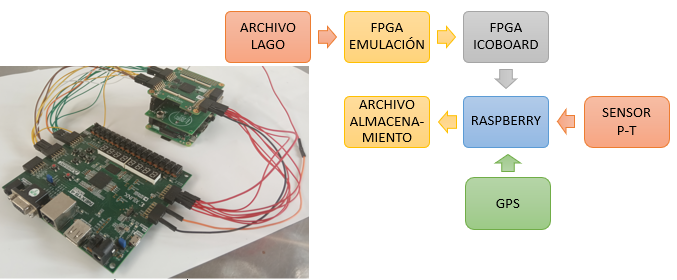
\includegraphics[width=1\textwidth]{Figs/verifica.png} 
\centering
\caption{Implementación para verificación de resultados}
\label{verifi}
\end{figure}

Para verificar las descripciones implementadas a nivel RTL se simularon los diseños originales del proyecto LAGO para ser comparadas con los actuales. Cabe resaltar que las simulaciones que se presentan a continuación , tienen como entrada una base de datos en representación binaria a 12 bits y formato \texttt{.mem}, la cual se genera con eventos extraídos de los archivos de salida obtenidos con la versión orginal del proyecto LAGO.
Dichos archivos han sido validados por el grupo de investigación Halley encargado del proyecto en Colombia.

\section{\textbf{Comparación simulaciones de LAGO}}

\begin{figure}[H]
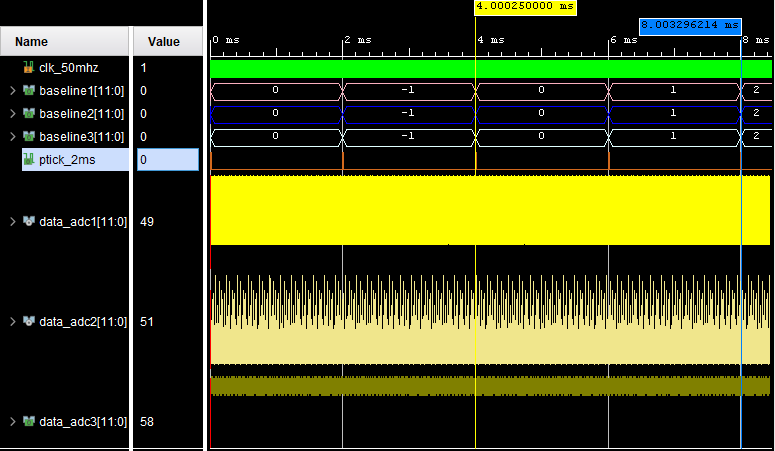
\includegraphics[width=0.9\textwidth]{Figs/actualbase.PNG} 
\centering
\caption{Simulación del comportamiento de las señales en baseline, versión actualizada}
\label{sim2ms}
\end{figure}

\subsection{Comparación simulación Baseline versión original y actualizada}
En la simulación mostrada en la Figura~\ref{sim2ms} en color café se muestra la actualización de la señal (ptick\_2ms) con un período de 2ms.

A cada canal de entrada (data\_adc1, data\_adc2, data\_adc3) se le ingresa una señal diferente desde la memoria del hardwware externo. Las señales de salida (baseline\_1, baseline\_2, baseline\_3), tienen el mismo comportamiento, ya que en el diseño se tiene un contador que acumula por 2 ms los datos provenientes de cada canal y calcula un promedio del error en la entrada con respecto a una referencia de 50 mV que en este caso corresponde a 50 niveles de cuantización. La salida de este circuito será conectada a un DAC para generar el voltaje necesario y así, corregir el offset de línea base para mantener el sistema en estado estable.  

%Así, se logra la estabilización de la linea base por los niveles de cuantización entregados al DAC.


\begin{figure}[H]
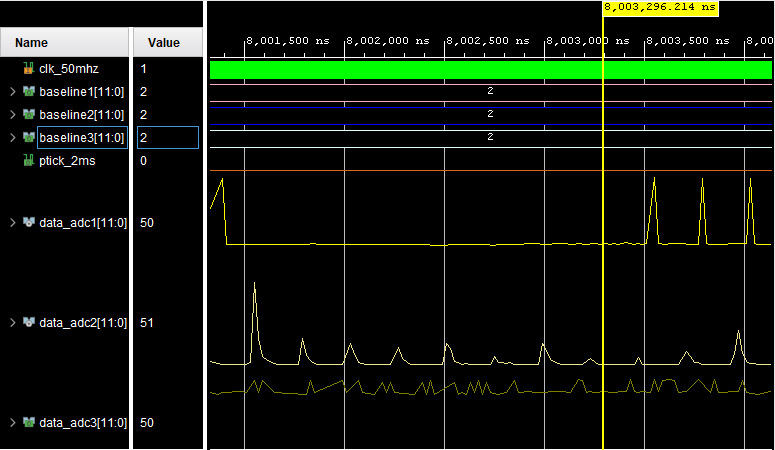
\includegraphics[width=0.9\textwidth]{Figs/zombasenue.PNG} 
\centering
\caption{Simulación de las entradas de baseline, versión actualizada}
\label{finbase}
\end{figure}

En la  Figura~\ref{finbase} se hace un acercamiento al cursor posicionado en 8,00329996214~ ms mostrado en la figura anterior, para observar el comportamiento de las entradas en forma análogica, nótese el  comportamiento diferente que tienen las tres entradas.

%\begin{itemize}
%    \item {\textbf{Simulación Baseline versión original}}
%\end{itemize}


El comportamiento en las señales de salida (baseline1, baseline2, baseline3) es similar logrando una actualización cada 2 ms.

%En la Figura~\ref{baseor}, el cursor amarillo se ubica en el mismo instante de tiempo que en Figura~\ref{finbase}, pero las entradas (data\_adc) no se encuentran en el mismo valor numerico que se presenta en la columna (value), eso se debe a la mejora en la frecuencia de la versión actualizada, que se implementa a 50 MHz con respeto a la original implementada a 40 MHz . De acuerdo a lo anterior los datos que se observan son diferentes, 



%se presentan las mismas señales del control de linea base con el fin de verificar el comportamiento similar, nótese algunas diferencias como el periodo de muestreo es de 25ns ya que se tiene una frecuencia menor y por tanto los datos que se observan en los cursores son diferentes. Sin embargo, el comportamiento de las salidas(baseline1, baseline2, baseline3) es similar y al igual se logra una actualización cada 2ms.
 
\begin{figure}[H]
\includegraphics[width=0.9\textwidth]{Figs/baselineori.PNG} 
\centering
\caption{Simulación del comportamiento de las señales en baseline, versión original}
\label{actu4ms}
\end{figure}

En la Figura~\ref{baseor}, el cursor amarillo se ubica en el mismo instante de tiempo que en Figura~\ref{finbase}, pero las entradas (data\_adc) no se encuentran en el mismo valor numerico que se presenta en la columna (value), eso se debe a la mejora en la frecuencia de la versión actualizada, que se implementa a 50 MHz con respeto a la original implementada a 40 MHz . De acuerdo a lo anterior los datos que se observan son diferentes.

\begin{figure}[H]
\includegraphics[width=0.9\textwidth]{Figs/zombase.PNG} 
\centering
\caption{Simulación de las entradas de baseline, versión original}
\label{baseor}
\end{figure}
%__________________________________________________________________________Seguir revisando 

\subsection{Comparación simulación rampa versión original y actualizada}
En esta simulación se evidencian algunos cambios realizados respecto al diseño original LAGO con el fin de aplicar unas mejoras. Una es la restricción del máximo valor que el usuario puede ingresar como parámetro de entrada DATA\_IN(1023) a la rampa.
Dado que en la versión original aunque el valor máximo efectivo es 1023, es posible ingresar un número mayor así no tenga efecto alguno en la generación de la señal de salida.

En la Figura~\ref{10ns} se puede observar las rampas que se generan a partir de tres valores de polarización que se ingresan en distintos instantes de tiempo por el usuario, con tiempo de 200 ms en estado estable para cada uno.

\begin{figure}[H]
\includegraphics[width=0.9\textwidth]{Figs/Rampa_100Mhz.PNG} 
\centering
\caption{Simulación rampa de polarización del proyecto LAGO, versión actualizada}
\label{10ns}
\end{figure}
En Figura~\ref{10ns2} se observa un acercamiento donde se puede apreciar el comportamiento del ciclo útil en la señal (PWM\_pulse) con duración de 20 ns.


\begin{figure}[H]
\includegraphics[width=0.9\textwidth]{Figs/zomnuevo.PNG} \centering
\caption{Ciclo útil de 10 ns para la PWM del proyecto LAGO, versión actualizada}
\label{10ns2}
\end{figure}


\begin{itemize}
    \item {\textbf{Simulación Rampa versión original}}
\end{itemize}

Para estimular este diseño se ingresa un \texttt{DATA\_IN} de 1023, de igual manera se estimula con un período de 20~ns ya que la frecuencia de la FPGA utilizada es de 50 MHz.
La salida (data\_out) cambia cada 4 ms como se muestra en la Figura~\ref{ciclo10}.

\begin{figure}[H]
\includegraphics[width=0.9\textwidth]{Figs/pwmoriginal.PNG} 
\centering
\caption{Actualización de la PWM del proyecto LAGO, versión original}
\label{actualizacionac}
\end{figure}

A diferencia del diseño original de LAGO este diseño tiene un ciclo útil de 20 ns lo cual se evidencia en logrando actualizar la PWM de manera más rápida.

\begin{figure}[H]
\includegraphics[width=0.9\textwidth]{Figs/zomviejo.PNG} 
\centering
\caption{Ciclo útil de 20ns para la PWM del proyecto LAGO, versión original}
\label{ciclo10}
\end{figure}

\begin{figure}[H]
 \centering
 \includegraphics[width=0.9\textwidth]{Figs/Rampa_50MHz.PNG}
 \caption{Ciclo útil de 20ns para la PWM del proyecto LAGO, versión original}
 \label{ramapa50}
\end{figure}

En la Figura~\ref{ramapa50} se estimula el circuito con las condiciones presentadas en la Figura~\ref{10ns}.

Las simulaciones evidencian que las dos versiones presentan el mismo tiempo de establecimiento el cual se puede ver en los cursores de la Figura~\ref{ramapa50} y la Figura~\ref{10ns}. De lo anterior podemos concluir que conserva la misma respuesta la señal de salida.



\subsection{Comparación simulación Trigger versión original y actualizada}
Las señales se estimulan con un reloj de periodo 20 ns.
%Se estimulan las señales con un periodo de 20ns, en la Figura~\ref{tigeer} El segmento extraido expone el funcionamento del circuito para la discriminación de datos llamado Trigger.

\begin{figure}[H]
\centering
\includegraphics[width=0.9\textwidth]{Figs/trigernevo.PNG} 
\caption{Señales de Trigger destacadas del proyecto LAGO, versión actualizada}
\label{tigeer}
\end{figure}

La simulación muestra el circuto en estado de detección que evidencia la secuencia de señales necesarias para el almacenamiento del evento considerado rayo cósmico. Ver Figura~\ref{tigeer}

La señal (s\_tr) se activa en el momento que cualquier canal de entrada (Data\_adc) supera sus respectivos umbrales (trigger\_set), dos ciclos de reloj después, se pone en alto (pwr\_enA) durante 340 ns indicando que se almacenarán las 15 muestras que ingresan de la captura.\\
La señal (data\_out) concatena las muestras de los tres canales para su posterior comunicación por protocolo SPI con la Raspberry Pi, de modo que se envían consecutivamente 15 tramas de datos correspondientes al evento y dos adicionales para los contadores (tr\_status\_reg) y (ctr\_status\_reg).


%, pwr\_enA se pone en alto cuando se tiene información para almacenar, a su vez se evidencia data\_out una señal de 38 bits entrega la información del evento en 340ns; 15 ciclos de muestras seguidos por 2 ciclos más que entregan los contadores(tr\_status\_reg) y (ctr\_status\_reg).
%Nótese además en esta figura la posibilidad de disparo(s\_tr) en cualquiera de los 3 canales ya que se establece el mismo umbral de activación en (trigger1, trigger2, trigger3),



%cabe resaltar el ingreso de valores diferentes en las  entradas(data\_adc1,data\_adc2,data\_adc3) y el cursor posicionado en 370ns para evidenciar la bandera de 2 bits y el registro de las muestras en los 3 canales en orden ascendente.

\begin{itemize}
    \item {\textbf{Simulación Trigger versión original}}
    
\end{itemize}

En  la Figura~\ref{trigerlago} cabe notar algunas diferencias que se presentan por las mejoras realizadas al diseño. Se estimularon las señales con un reloj de 40 MHz, Data\_out se respresenta en 32 bits, el tiempo en que pwr\_enA esta en alto de 350 ns. Al igual que la figura anterior se establecen los mismo estímulos de entrada para evidenciar un comportamiento similar en los diseños.
\begin{figure}[H]
\includegraphics[width=0.9\textwidth]{Figs/trigerviejo.PNG} 
\centering
\caption{Señales de Trigger destacadas del proyecto LAGO, versión original}
\label{trigerlago}
\end{figure}

Como se evidencia en cada una de las simulaciones se logra obtener un resultado equivalente en las señales de control que componen el procesamiento de datos del proyecto LAGO y algunas mejoras como el aumento en la frecuencia de muestreo.

\section{\textbf{Salida de control para PMT's}}
A continuación se muestran graficas de la señal PWM obtenida luego de implementar en FPGA los diseños expuestos en Capítulo 3.

\begin{figure}[H]
\includegraphics[width=0.9\textwidth]{Figs/PWM 2.jpeg} 
\centering
\caption{Señal de control PWM, versión actualizada}
\label{pwmactual}
\end{figure}
\begin{figure}[H]

\includegraphics[width=0.9\textwidth]{Figs/TEK00019.PNG} 
\centering
\caption{Señal de control PWM, versión actual}
\label{pwmantigua}
\end{figure}


En la Figura ~\ref{pwmactual} se obtiene una señal que cumple con una frecuencia medida en osciloscopio de 9,823 KHz de ciclo útil variable y un voltaje máximo de 2,714 V.

En la Figura~\ref{pwmantigua} se observa la señal PWM en el CH2 con un período de 102,3 us equivalente a una frecuencia de 9,775 KHz con un ciclo útil varible.


\section{\textbf{Registro de datos}}
En primer lugar se resalta la terminal de usuario Figura~\ref{adecuacion} en la que se ingresan cada uno de los umbrales ya explicados durante el desarrollo del proyecto.

%En esta terminal se hacen algunas abreviaturas de las constantes que pueden aparecer duante el registro y el almacenamiento de la información.

\begin{figure}[H]
\includegraphics[width=0.95\textwidth]{Figs/terminal.PNG} 
\centering
\caption{Cabecera del archivo de datos del terminal de usuario proyecto LAGO}
\label{adecuacion}
\end{figure}

Luego de la implementación se obtiene el siguiente archivo de salida en el cual se evidencia la correcta comunicación entre la Icoboard y la Raspberry Pi para registrar el evento proveniente de la FPGA Nexys 4 a una frecuencia de 50 MHz. 

En la Figura~\ref{mta} se muestra en recuadro rojo un recorte de uno de los eventos obtenidos en el archivo de salida como resultado de este proyecto, y en recuadro azul un recorte de uno de los eventos tomado como referencia del proyecto LAGO. 

\begin{figure}[H]
\includegraphics[scale=0.9]{Figs/eventos.PNG} 
\centering
\caption[Comparación de archivos de salida con datos de eventos considerados rayos cósmicos]{Comparación de archivos de salida con datos de eventos considerados rayos cósmicos. *\textbf{Cuadro rojo:} versión actualizada. *\textbf{Cuadro azul:}versión original}
\label{mta}
\end{figure}


En la Figura~\ref{adecuacion} se muestra un evento para corrobar el funcionamiento del diseño implementado y mostrar el comportamiento de los datos obtenidos, además, una interpolación de las muestras registradas usando Matlab~\textregistered~ para tener un acercamiento real de la forma del pulso de un evento considerado rayo cósmico.

\begin{figure}[H]
\includegraphics[width=0.9\textwidth]{Figs/salidadata.jpeg} 
\centering
\caption[Gráfica de evento hardware vs pulso interpolado]{(Arriba) Gráfica discreta de un evento registrado por el hardware diseñado.(Abajo) pulso interpolado}
\label{adecuacion}
\end{figure}

Con el sistema de adquisición implementado se tomaron datos de presión y temperatura durante media hora los cuales se muestran en las siguientes graficas, estos datos son importantes en el proyecto LAGO ya que mediante análisis de estos datos se logra hacer correcciones en los detectores WCD. 


\begin{figure}[H]
\includegraphics[width=0.9\textwidth]{Figs/TEMPERATURA.PNG} 
\centering
\caption{Registro de temperatura HP03S durante un registro de media hora}
\label{temp}
\end{figure}

\begin{figure}[H]
\includegraphics[width=0.9\textwidth]{Figs/presion.PNG} 
\centering
\caption{Registro de presión HP03S durante un tiempo de registro de media hora}
\label{pre}
\end{figure}

Con el sistema de adquisición implementado se tomaron datos de presión y temperatura durante media hora los cuales se muestran en estas graficas, estos datos son importantes en el proyecto Lago ya que mediante análisis de estos datos se logra hacer correcciones en los detectores WCD. 

Finalmente con el diseño descrito durante el desarrollo del proyecto se logra optimizar el sistema de adquisición para dar soporte y continuidad al proyecto implementando una lógica distinta a la del proyecto LAGO, mejorando la compatibilidad con los dispositivos para almacenar información relevante de los periféricos HP03S y GPS. Mediante herramientas de desarrollo libres como Yosys, Arachne, Icepack y Iceprog se logra la independencia respecto a las FPGA en el proyecto. 

% ------------------------------------------------------------------------    % Resultados
%% ------------------------------------------------------------------------
% ------------------------------------------------------------------------
% ------------------------------------------------------------------------
%                            Recomendaciones
% ------------------------------------------------------------------------
% ------------------------------------------------------------------------
% -----------------------------------------------------------------------
% ------------------------------------------------------------------------    % Recomendaciones
% ------------------------------------------------------------------------
% ------------------------------------------------------------------------
% ------------------------------------------------------------------------
%                            Trabajo futuro
% ------------------------------------------------------------------------
% ------------------------------------------------------------------------
% ------------------------------------------------------------------------

\chapter{Trabajo futuro}

Para dar por terminada la actualización del sistema de adquisición del proyecto LAGO se debe aplicar una mejora a la electrónica analógica, aumentando la frecuencia de muestreo y la resolución para adaptarlo a la implementación de este proyecto.

% ------------------------------------------------------------------------

% ------------------------------------------------------------------------    % Trabajo futuro
% ------------------------------------------------------------------------
% ------------------------------------------------------------------------
%                             Conclusiones
% ------------------------------------------------------------------------
% ------------------------------------------------------------------------

\chapter{Conclusiones}
% Se presenta en forma exacta el aporte del desarrollo den trabajo en concordancia a la justificación presentada.
% Se describe en forma lógica, los resultados del trabajo, dando respuesta a los objetivos o propósitos planteados.
% Basado en los resultados recolectados, incluido el tratamiento estadístico o cualitativo.
% Se muestra en forma concisa los productos y/o resultados y se resaltan las contribuciones del trabajo al contexto local, regional, nacional e internacional, cuando aplique.

% ------------------------------------------------------------------------
En este proyecto se diseñó un sistema de preprocesamiento digital para el registro de aquellos eventos que pueden ser considerados rayos cósmicos, se implementaron circuitos a nivel RTL en una FPGA con herramientas libres, esta versión obedece a una actualización del proyecto LAGO mejorando la frecuencia de muestreo del evento captado de 40~MHz a 50~MHz y conservando el comportamiento en las señales de control.
    
Se almacena la información de lo eventos registrados en una Raspberry Pi3 model B+ comunicada con la FPGA Icoboard por medio de protocolo SPI, además se registró los datos de los periféricos HP03S y GPS que permiten obtener información relacionada con el entorno del WCD (ubicación geográfica, hora, temperatura ambiente y presión atmosférica).


% -------------------------------------------------------------------
   % Conclusiones
% ------------------------------------------------------------------------
% Bibliografía
% ------------------------------------------------------------------------
\addcontentsline{toc}{chapter}{Referencias}\newpage
\bibliographystyle{apalike}
\bibliography{xbib}
% ------------------------------------------------------------------------
% Anexos
% ------------------------------------------------------------------------
%% ------------------------------------------------------------------------
% ------------------------------------------------------------------------
% ------------------------------------------------------------------------
%                                Anexo A
% ------------------------------------------------------------------------
% ------------------------------------------------------------------------
% ------------------------------------------------------------------------
% ------------------------------------------------------------------------
\newpage
\nnchapter{Apéndices}
% ------------------------------------------------------------------------
\anexo{Fundamentos de sólidos rígidos}\label{anexoA}
% ------------------------------------------------------------------------
\noindent Un sólido rígido, es un cuerpo formado por varias partículas puntuales que
guardan distancias constantes entre sí \citep{sears2005fisica}.\\

Una operación fundamental para definir cantidades en el espacio de movimiento de
un sólido rígido es el producto vectorial (también denominado producto cruz \citep{stanley1993algebra}),
el cual produce un vector perpendicular (normal) al plano formado por otros dos vectores
que se multiplican.\\

Sean dos vectores $\vec{a}$ y $\vec{b}$ definidos en $\mathbb{R}^3$. El producto vectorial entre $\vec{a}$ y $\vec{b}$ (denotado $\vec{a} \times \vec{b}$) es otro vector (digamos $\vec{c} \in \mathbb{R}^3$) cuyo cálculo puede ser efectuado a través de determinantes como sigue:
% ------------------------------------------------------------------------
\begin{equation}\label{defprodvect}
\vec{c} = \vec{a} \times \vec{b} = \begin{vmatrix}
i& j & k \\
a_i & a_j  & a_k \\
b_i & b_j  & b_k
\end{vmatrix} =
\begin{vmatrix}
 a_j & a_k \\
 b_j & b_k
\end{vmatrix}i~
-
\begin{vmatrix}
a_i & a_k \\
b_i & b_k
\end{vmatrix}j~
+\begin{vmatrix}
 a_i & a_j \\
 b_i & b_j
\end{vmatrix}k
\end{equation}
% ------------------------------------------------------------------------
De esta manera, siendo $\vec{a}=(1,-1,2)$ y $\vec{b}=(3,-4,5)$ se obtiene:
% ------------------------------------------------------------------------
\begin{equation}
\vec{a} \times \vec{b} =\begin{vmatrix}
i& j & k \\
1 &-1  &2 \\
3 &-4  &5
\end{vmatrix}=
\begin{vmatrix}
 -1&2 \\
 -4&5
\end{vmatrix}i~
-
\begin{vmatrix}
1 &2 \\
3 &5
\end{vmatrix}j~
+\begin{vmatrix}
 1&-1 \\
 3&4
\end{vmatrix}k
= 3i-j-k
\end{equation}
% ------------------------------------------------------------------------
La Fig. \ref{prodvect} ilustra esta operación gráficamente en el espacio tridimensional.
% ------------------------------------------------------------------------
\begin{figure}[h]
\centering
\includegraphics[width=0.3\textwidth]{Figs/prodvect}
\caption[]{Ilustración gráfica para producto vectorial}\label{prodvect}
\end{figure}
% ------------------------------------------------------------------------

\section*{Condición de rigidez}
% ------------------------------------------------------------------------
\noindent Considere el sólido rígido presentado en la Fig. \ref{rigid}. Para cada pareja de puntos $(P_i, P_j)$ pertenecientes al sólido, se cumple:
% ------------------------------------------------------------------------
\begin{equation}\label{rigidez}
\frac{d}{dt}[\left|r_i - r_j\right|] = \frac{d}{dt}[\left|r_{ij}\right|] = 0,
\end{equation}
% ------------------------------------------------------------------------
lo cual significa que la distancia entre puntos de un sólido rígido se mantiene invariante. Esto último se conoce como la \emph{condición de rígidez}.\\
% ------------------------------------------------------------------------
\begin{figure}[h]
\centering
\includegraphics[width=0.3\textwidth]{Figs/rigid}
\caption[]{Sólido rígido}\label{rigid}
\end{figure}
% ------------------------------------------------------------------------

Asimismo, a partir de \eqref{rigidez} se obtiene:
% ------------------------------------------------------------------------
\begin{equation}
\frac{d}{dt}[\left|r_i - r_j\right|] = \left|\dot{r}_i - \dot{r}_j\right| = 0,
\end{equation}
% ------------------------------------------------------------------------
y por tanto, sabiendo que $\vec{\dot{r}}$ es el vector velocidad $\vec{v}$ para un punto del sólido visto desde el observador, es posible escribir:
% ------------------------------------------------------------------------
\begin{equation}
\left|v_i\right| = \left|v_j\right|,
\end{equation}
% ------------------------------------------------------------------------
con lo cual la velocidad de traslación para cualquier punto del sólido será la misma, y así, una vez definido el movimiento de un punto cualquiera del cuerpo rigido que se traslada en el espacio, es posible definir la totalidad de su movimiento.

% ------------------------------------------------------------------------
\section*{Movimiento de rotación}
% ------------------------------------------------------------------------
\noindent En la Fig. \ref{rotacion} se ilustra un punto que rota alrededor de un eje fijo, localizado en el cuerpo del sólido.\\
% ------------------------------------------------------------------------
\begin{figure}[h]
\centering
\includegraphics[width=0.3\textwidth]{Figs/rotacion}
\caption[]{Rotación de un punto del sólido alrededor de un eje fijo}\label{rotacion}
\end{figure}
% ------------------------------------------------------------------------

A partir de ello, es posible definir la velocidad angular que experimenta el punto $P$ alrededor del eje de rotación, en el modo siguiente:
% ------------------------------------------------------------------------
\begin{equation}
\omega = \frac{d}{dt}\theta
\end{equation}\
% ------------------------------------------------------------------------

Tambien, puede escribirse del diagrama la velocidad tangencial $v$ del punto mediante:
% ------------------------------------------------------------------------
\begin{equation}
\vec{v} = \vec{r} \times \vec{\omega},
\end{equation}
% ------------------------------------------------------------------------
siendo $\vec{r}$ el vector que marca la distancia del punto $P$ al eje de rotación $O$.\\

Por tanto, el vector de aceleración puede ser formulado como:
% ------------------------------------------------------------------------
\begin{eqnarray}\label{aceler}
\nonumber \frac{d}{dt}\vec{v} & = & \frac{d}{dt}[\vec{r} \times \vec{\omega}]\\
\nonumber & = & \left( \frac{d}{dt}\vec{r}\times \vec{\omega}\right) + \left( \vec{r}\times \frac{d}{dt}\vec{\omega}\right)\\
\vec{a}   & = & \vec{r} \times \vec{\alpha},
\end{eqnarray}
% ------------------------------------------------------------------------
con $\vec{a}$ y $\vec{\alpha}$ representando, respectivamente, los vectores de aceleración lineal y angular. Note que se asume $\frac{d}{dt}\vec{r} = 0$ debido a que el eje de rotación es fijo.

% ------------------------------------------------------------------------
\section*{Conservación del momento angular}
% ------------------------------------------------------------------------
\noindent En un movimiento traslacional, el principio de conservación del momento lineal establece:
% ------------------------------------------------------------------------
\begin{equation}
\frac{d}{dt}\vec{p} = \frac{d}{dt}{m\vec{v}} = 0,
\end{equation}
% ------------------------------------------------------------------------
a partir de lo cual el momento $\vec{p}$ será constante en ausencia de fuerzas externas.\\

De manera similar, es posible definir el momento angular $\vec{\mathbf{L}}$ de una partícula de masa puntual que rota alrededor de un eje fijo, en el modo siguiente:
% ------------------------------------------------------------------------
\begin{equation}\label{momang}
\vec{\mathbf{L}} = \vec{r} \times \vec{p},
\end{equation}
% ------------------------------------------------------------------------
siendo $\vec{r}$ el vector de distancia a la masa desde el centro de rotación.\\

Por tanto, el principio de conservación del momento angular puede establecerse como sigue:
% ------------------------------------------------------------------------
\begin{eqnarray*}
\frac{d}{dt}\vec{\mathbf{L}} & = & \frac{d}{dt}{[\vec{r} \times \vec{p}]} \\
                             & = & \frac{d}{dt}{[\vec{r} \times m\vec{v}]}\\
                             & = & m \frac{d}{dt}{[\vec{r} \times \vec{v}]}\\
                             & = & m\left([\vec{r}\times\frac{d}{dt}\vec{v}]+[\frac{d}{dt}\vec{r}\times\vec{v}]\right)\\
                             & = & m\left([\vec{r}\times \vec{a}]+[\vec{v}\times\vec{v}]\right)\\
                             & = & \vec{r}\times m\vec{a}\\
                             & = & \vec{r}\times \vec{F}\\
                             & = & \tau,
\end{eqnarray*}
% ------------------------------------------------------------------------
siendo $\tau$ el torque neto aplicado.\\

Empleando \eqref{aceler} puede relacionarse este torque con la aceleración angular $\vec{\alpha}$, a partir de:
% ------------------------------------------------------------------------
\begin{eqnarray*}
\tau & = & \vec{r}\times m\vec{a}\\
     & = & \vec{r}\times m\left(\vec{r} \times \vec{\alpha}\right)\\
     & = & m\left(\vec{r}\times \left(\vec{r} \times \vec{\alpha}\right)\right)
\end{eqnarray*}
% ------------------------------------------------------------------------
donde, si $\vec{r}$ es perpendicular a $\vec{\alpha}$, entonces el producto vectorial se reduce al producto de las magnitudes:
% ------------------------------------------------------------------------
\begin{eqnarray}\label{newrot}
\nonumber \tau & = & m r^2 \alpha \\
               & = & I \alpha,
\end{eqnarray}
% ------------------------------------------------------------------------
siendo $I$ el momento de inercia de las partes rotativas del cuerpo rígido.\\

La expresión \eqref{newrot} es la segunda ley de Newton de rotación, y podrá ser definida siempre que sea válido un $I$ constante. Dicha situación no siempre es posible, principalmente si se asume que el eje de rotación puede variar en el tiempo. En tal caso, $\vec{r}$ en la Fig. \ref{rotacion} no es constante y por tanto no es válida la solución propuesta para $\vec{a}$ en \eqref{aceler}, resultando en la siguiente definición alternativa para $\tau$:
% ------------------------------------------------------------------------
\begin{eqnarray*}
\tau & = & \vec{r}\times m\vec{a}\\
     & = & \vec{r}\times m\left(\left( \frac{d}{dt}\vec{r}\times \vec{\omega}\right) + \left( \vec{r}\times \frac{d}{dt}\vec{\omega}\right)\right)\\
     & = & m\left(\left[\vec{r}\times\left( \frac{d}{dt}\vec{r}\times \vec{\omega}\right)\right] + \left[\vec{r}\times\left( \vec{r}\times \vec{\alpha}\right)\right]\right)\\
     & = & m\left(\left[\vec{r}\times\left( \frac{d}{dt}\vec{r}\times \vec{\omega}\right)\right]\right) + I\alpha.
\end{eqnarray*}\
% ------------------------------------------------------------------------

El término
% ------------------------------------------------------------------------
$$
m\left(\left[\vec{r}\times\left( \frac{d}{dt}\vec{r}\times \vec{\omega}\right)\right]\right),
$$\
% ------------------------------------------------------------------------
representa los efectos (torques) debidos a las variaciones del eje de rotación, que evidentemente también representan variaciones del vector de momento angular $\vec{\mathbf{L}}$. Dichos efectos se denominan \emph{fuerzas inerciales}, puesto que tienen sentido en un marco de referencia de un cuerpo en rotación. Los tipos más representativos de fuerza inercial son los efectos giroscópicos y la fuerza de Coriollis \citep{sears2005fisica}.
% ------------------------------------------------------------------------  % Fundamentos de sólidos rígidos
%% ------------------------------------------------------------------------
%                                Anexo B
% ------------------------------------------------------------------------
\newpage
\anexo{Función \emph{ode45} de MATLAB}\label{anexoB}
% ------------------------------------------------------------------------
\noindent La función $ode45$ está basada en un algoritmo de tipo Runge-Kutta, que se desarrolló a partir del método de Euler mejorado \citep{chapra2003metodos}. La función recibe tres parámetros esenciales: $f(t)$ dentro de un $script$ en el que se define la ecuación diferencial acompañado por un simbolo $@$, el vector de límites de tiempo $\left[ t_0 \quad t_f \right]$ y el vector de condiciones iniciales $y_0$. En otras palabras el prototipo básico para usar \emph{ode45} es el siguiente:
% ------------------------------------------------------------------------
\begin{equation}\label{defode}
   [t,y]=\emph{ode45}(@f(t),\left[ t_0 \quad t_f \right],y_0);
    \end{equation}
% ------------------------------------------------------------------------
En este caso la solución numérica se almacenará en el vector $y$  para cada uno de los instantes de tiempo presentes en el vector $t$.\\

La función $ode45$, resuelve ecuaciones del tipo $\dot{y} = f(t,y)$, por tanto si se desea resolver ecuaciones de orden superior estas deben escribirse como un sistema de ecuaciones diferenciales de primer orden.\\

A manera de ejemplo, se ilustrará la forma de resolver la ecuación diferencial de segundo orden
% ------------------------------------------------------------------------
\begin{equation}\label{segundo}
   \ddot{x}-\mu\left(1-x^2\right)\dot{x}+x=0,
\end{equation}
% ------------------------------------------------------------------------
donde $\mu > 0$ es un parámetro escalar.\\

Por tanto, definiendo
% ------------------------------------------------------------------------
$$y_1 = x; \quad y_2 = \dot{x}$$
% ------------------------------------------------------------------------
la expresión \eqref{segundo} puede ser reescrita como
% ------------------------------------------------------------------------
$$
\dot{y}_2 = \mu \left( 1 - y_1^2 \right) y_2 + y_1
$$
% ------------------------------------------------------------------------
es decir, transformando la ecuación diferencial original de segundo orden y una variable, en una ecuación diferencial equivalente de primer orden y dos variables. Así entonces, es posible construir el vector
% ------------------------------------------------------------------------
$$
y = \left[ {\begin{array}{*{20}c}
   y_1  \\
   y_2  \\
\end{array}} \right]
$$
% ------------------------------------------------------------------------
cuya dinámica viene representada por
% ------------------------------------------------------------------------
$$
\dot{y} = \left[ {\begin{array}{*{20}c}
   f_1 \left(t, y \right)  \\
   f_2 \left(t, y \right) \\
\end{array}} \right]
$$
% ------------------------------------------------------------------------
siendo
% ------------------------------------------------------------------------
$$f_1\left(t, y \right) = y_2; \quad f_2\left(t, y \right) =  \mu \left( 1 - y_1^2 \right) y_2 + y_1$$
% ------------------------------------------------------------------------
De esta manera, evaluar la expresión \eqref{defode} permite obtener una matriz de salida $y$ con filas representando los vectores solución para $y_1$ e $y_2$ como función de $t$.\\
% ------------------------------------------------------------------------

\begin{figure}[h]
\centering
\includegraphics[width=0.55\textwidth]{Figs/flujodiag}
\caption[]{Diagrama de flujo para algoritmo de integración numérica de la función $ode45$ de MATLAB}\label{flujodiag}
\end{figure}
% ------------------------------------------------------------------------

En la Fig. \ref {flujodiag} se ilustra el diagrama de flujo del algoritmo empleado para hallar la solución de una ecuación diferencial mediante integración numérica empleando la función $ode45$ de MATLAB.\\

Inicialmente, se deben asignar los parámetros definidos en la ecuación \eqref{defode}.\\

Posteriormente, un bucle interno hace llamado iterativo a la función $f(t)$ evaluada para valores de tiempo entre $t_0$ y $t_f$ a partir de las condiciones iniciales $y_0$. Para cada ciclo la condición inicial se recalcula siendo la condición final del ciclo anterior. El tiempo se incrementa en un tamaño de paso $\delta t$ de forma adaptativa, si no se especifica lo contrario. Tras alcanzarse el tiempo final $t_f$, el bucle interno termina y entrega como resultado el vector de puntos de la trayectoria solución $y(t)$ al igual que el vector de tiempos $t$.  % Función ode45 de MATLAB
%\input{Secs/anexoC} % Interfaz de animación de la dinámica del sistema
% ------------------------------------------------------------------------
\end{document}                                          % Fin de documento
% ------------------------------------------------------------------------